\documentclass[a4paper,9pt]{article}
\usepackage[utf8]{inputenc}
\usepackage[margin=1in]{geometry}
\usepackage{graphicx}
\usepackage{titlesec}
\usepackage{caption}
\usepackage{hyperref}
\usepackage{float}
\usepackage{array}
\usepackage{chngcntr}
\counterwithin{figure}{section}
\renewcommand{\arraystretch}{2}
% Font and formatting settings
\usepackage{times}
\setlength{\parindent}{0pt}
\setlength{\parskip}{1em}
\titleformat{\section}{\large\bfseries\uppercase}{\thesection.}{1em}{}
\titleformat{\subsection}{\normalsize\bfseries\itshape}{\thesubsection.}{1em}{}
\titleformat{\subsubsection}{\normalsize\bfseries}{\thesubsubsection.}{1em}{}

% Page numbering
\pagestyle{plain}

\begin{document}
	
	% Title Page
	\begin{titlepage}
		\centering
		{\Huge\bfseries National University of Computer and
			Emerging Sciences\par}
		\vspace*{1cm}
		\begin{figure}[H]
			\centering
			
\includegraphics[width=0.62\linewidth]{fastlogo.png}
			\label{fig:enter-label}
		\end{figure}
		\vspace{1.6cm}
		{\Huge\bfseries\underline{Lab Manual ICT}\par}
		\vspace{1.3cm}
		
		\begin{table}[H]
			{\LARGE
				\hspace*{-1.3cm}
				\begin{tabular}{|p{4.4cm}|p{13.4cm}|} % Table with custom column widths
					\hline
					\textbf{Submitted By} & Mushaf Ali Mir \\ \hline
					\textbf{Session}      & Fall 2024 \\ \hline
					\textbf{Reg. No}      & 24P-0582 \\ \hline
					\textbf{Marks}        & \begin{tabular}[t]{@{}p{6cm}|p{4cm}@{}} % Nested table
						\textbf{Total: 5} & \textbf{Obtained:} \\
					\end{tabular} \\ \hline
				\end{tabular}
			}
			
		\end{table}
		
	\end{titlepage}
	
	\newpage
	\section*{\LARGE Declaration}
{\Large	I \underline{\textbf{Mushaf Ali Mir}} under registration number \underline{\textbf{24P-0582}} hereby declare that this Lab Assessment for ICT is entirely my own original work. I have not copied any part of this submission from any other source or individual. Should any similarity or plagiarism be found in this document, I acknowledge that I will be held responsible for academic dishonesty and will be subject to the disciplinary actions outlined in the academic rules of FAST University.}

\vspace{17cm}
	
	\textbf{\underline{\Large Checked By}:} \rule{4cm}{0.7mm}
	\vspace{0.7cm}
	
	\textbf{\underline{\Large Date}:} \rule{4cm}{0.5mm}
	
	\newpage
	\section*{\LARGE List Of Experiments}
	
	\setcounter{tocdepth}{1}
	\tableofcontents
	
	\newpage
	\begin{center}
		 \hspace*{-1.2cm}
	{\Huge \bfseries \underline{ LAB ASSESSMENT 1: Windows 11 Setup} \par}
	\end{center}
	\noindent\begin{tabular}{@{}ll}
		\textbf{Lab title} :& Installing Windows 11\\
		\textbf{Course name} :&  Introduction to Information and Communication Technology\\
		\textbf{Author name} : & Mushaf Ali Mir\\
		\textbf{Submission date} :& 2 Sept 2024 \\
	\end{tabular}
	
	\section*{Introduction}
	\addcontentsline{toc}{section}{1.   \hspace{1mm}Lab Task 1}
	\addtocounter{section}{1}
	
	Windows 11, the latest operating system from Microsoft, introduces a sleek user interface, enhanced productivity tools, and improved performance features. This experiment is designed to explore the key functionalities, settings, and practical applications of Windows 11, providing insights into its usability and system improvements.
	
	\subsection{Objective}
	The objective of this experiment is to understand the features and capabilities of Windows 11, explore its user interface, and perform various tasks to evaluate its functionality and performance in comparison to previous versions.
	\subsection{Apparatus/Materials}
\begin{enumerate}
	\item A computer or laptop compatible with Windows 11
	\item Windows 11 operating system installed
	\item Stable internet connection
	\item External storage device (e.g., USB or external hard drive).
	\item Basic computer accessories (keyboard, mouse, monitor)
	
\end{enumerate}
	\subsection{Theory}
	Windows 11 is built on the foundation of Windows 10, offering a modernized Start menu, enhanced multitasking features such as Snap Layouts, and improved gaming performance via DirectStorage. Understanding its design and features requires knowledge of operating system concepts, such as user interfaces, file management, system settings, and task management.
	
	\subsection{Procedure}
	\begin{enumerate}
		\item \textbf{Windows 11 Installation Setup:}
		
		\begin{figure}[H]
			\centering
			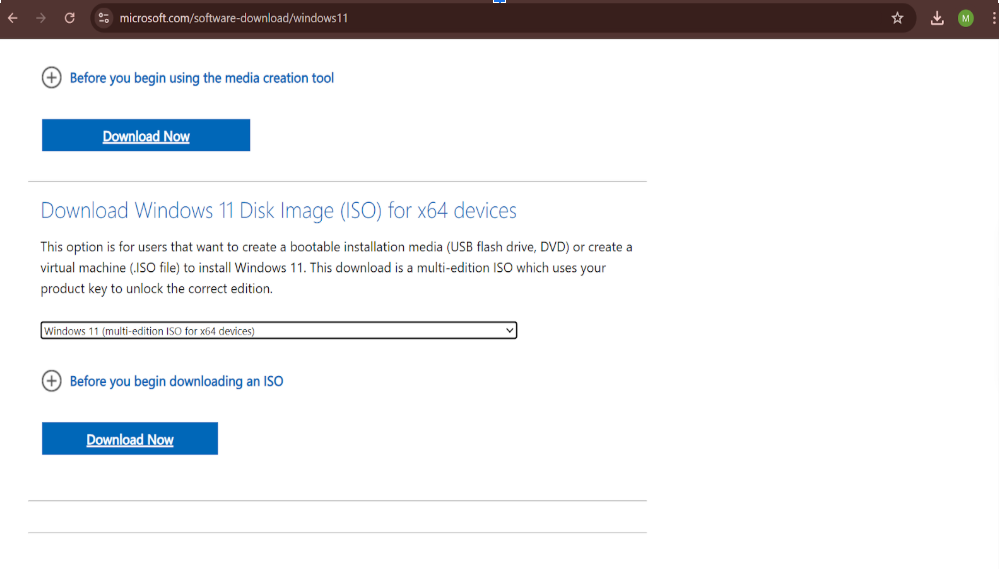
\includegraphics[width=0.8\linewidth]{1.1.png}
			\caption{Download Setup}
		\end{figure}
		STEP 1:-Download Windows 11 ISO file from microsoft official website
		https://www.microsoft.com/software-download/windows11 and Rufus from https://rufus.ie/en/,The purpose of rufus is to make our usb bootable so we can boot the iso file of windows 11 and install the windows
		\begin{figure}[H]
			\centering
			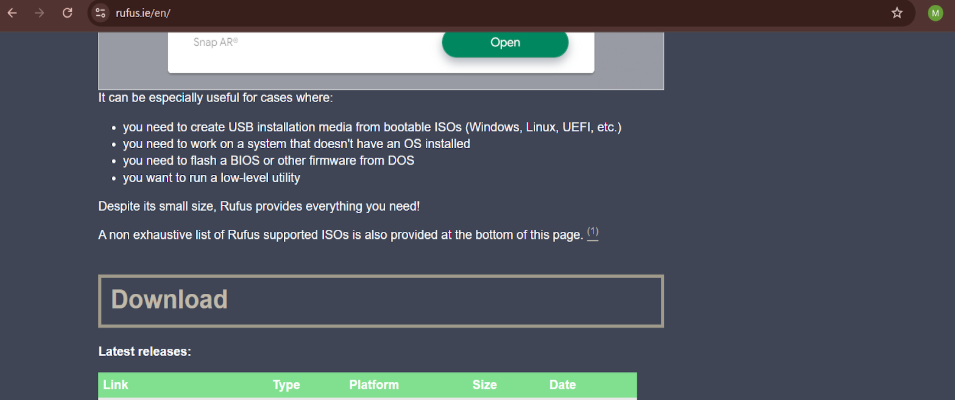
\includegraphics[width=0.8\linewidth]{1.2.png}
			\caption{Downloading Rufus}
		\end{figure}
		STEP 2:-Now we need to Plug our usb in our device and open the rufus software in the software we will select our usb in the device option and on the boot selection option we will select our iso file in the download directory and on the partition scheme we select GPT and target system UEFI and then click START and wait for the status to reach 100% and Close rufus
		
			\begin{figure}[H]
			\centering
			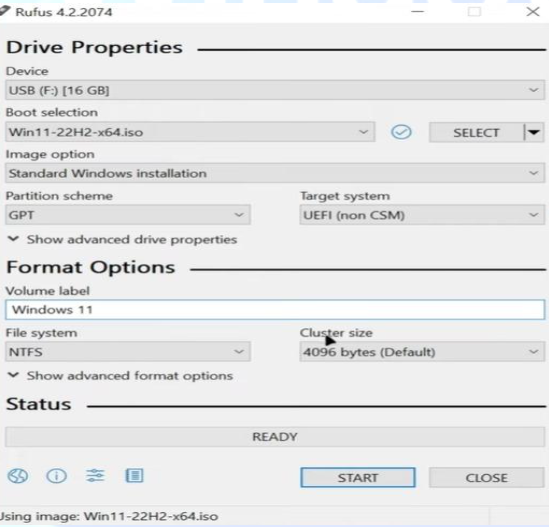
\includegraphics[width=0.8\linewidth]{1.3.png}
			\caption{Setup Rufus}
		\end{figure}
		STEP 3:-Now we will restart the system and upon reaching the system company logo we will open the boot menu by (Esc) and select our USB as 1st Priority and exit from the bios,after restart our system will reach the windows installation setup,select English
		
		\item \textbf{Windows 11 Installation:} 
			\begin{figure}[H]
			\centering
			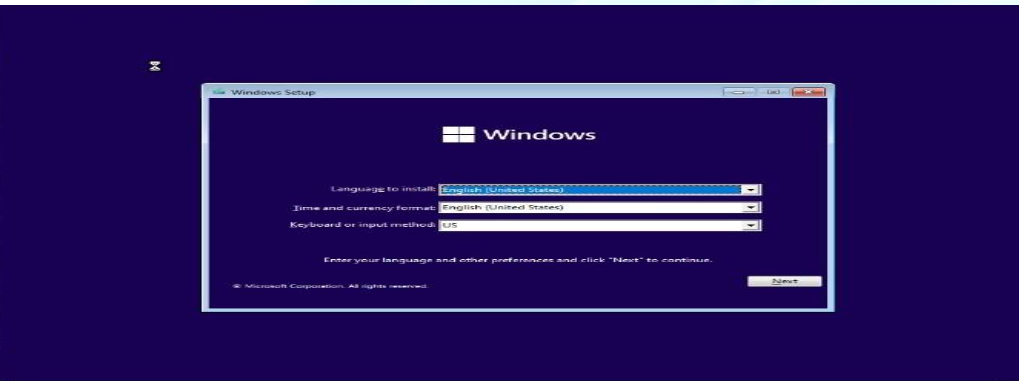
\includegraphics[width=0.8\linewidth]{1.4.png}
			\caption{Windows Installation}
		\end{figure}
		STEP 4:-Now we will select our preferred version of Windows 11,Personally i would select Windows 11 Home x64.
			\begin{figure}[H]
			\centering
			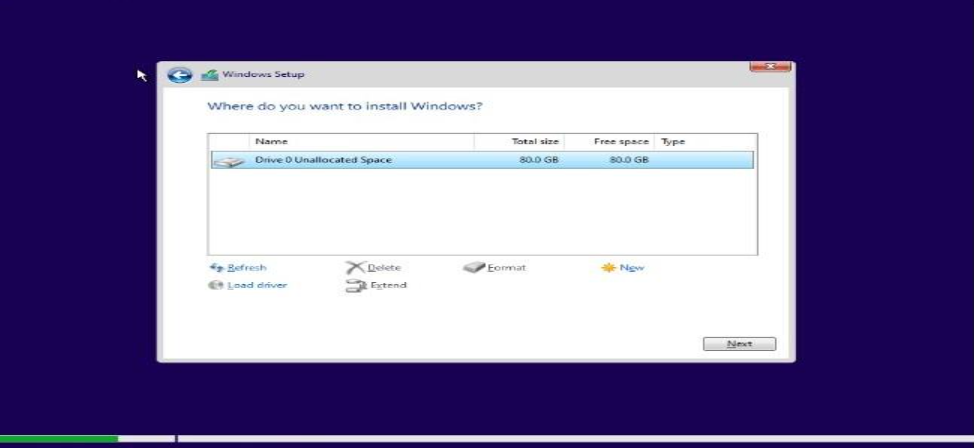
\includegraphics[width=0.8\linewidth]{1.5.png}
			\caption{Disk Partition}
		\end{figure}
		STEP 5:-Now we will select our preferred Windows Installation Type we can either select upgrade or custom we will select custom to install on our desired partition.
			\begin{figure}[H]
			\centering
			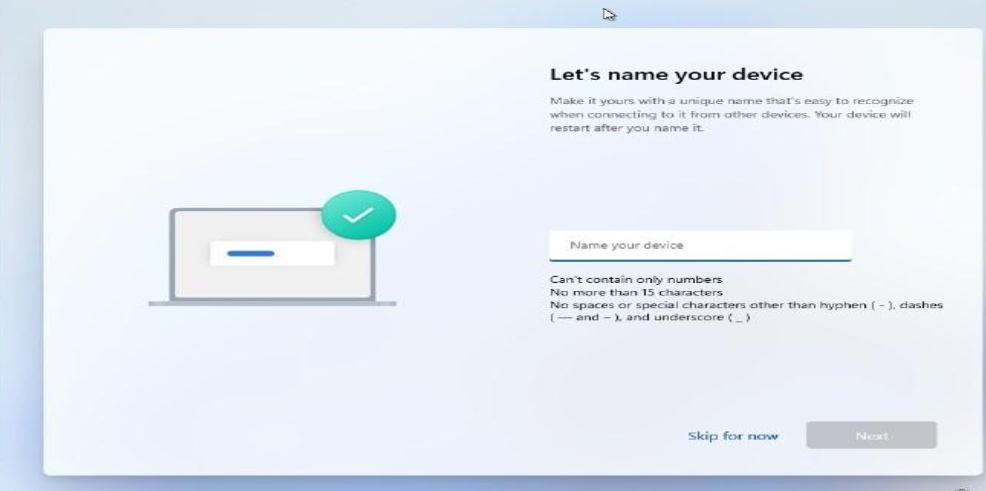
\includegraphics[width=0.8\linewidth]{1.6.png}
			\caption{Setting Name For Device}
		\end{figure}
		STEP 6:-Now we will name our device any preferred name can be used.
			\begin{figure}[H]
			\centering
			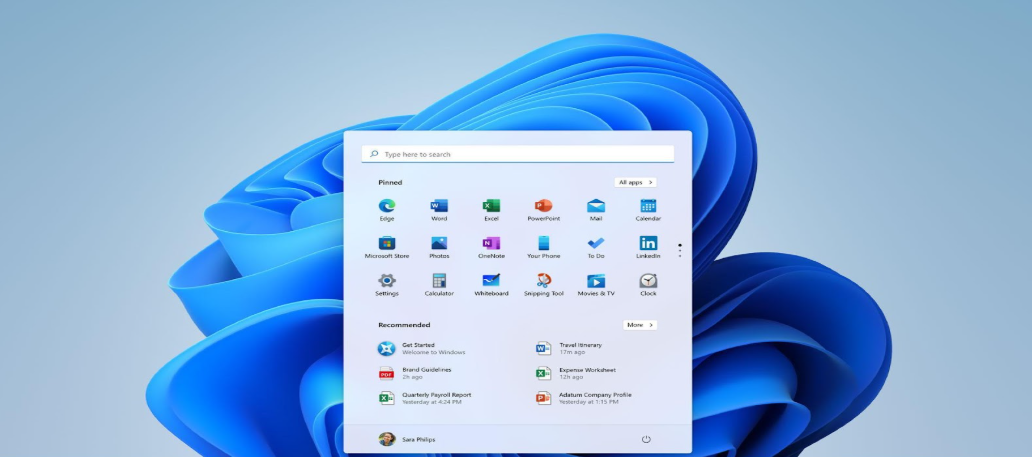
\includegraphics[width=0.8\linewidth]{1.7.png}
			\caption{Windows Setup Complete}
		\end{figure}
	   STEP 7:-	Now after some minutes we will be able to login in  our Windows 11.
	\end{enumerate}
	
	\subsection{Lab Task}
	
	\begin{itemize}
		\item Test and configure virtual desktops for productivity.
		\item Install and uninstall an application
		\item Test and configure virtual desktops for productivity.
		 
	\end{itemize}
	
	\subsection{Observation}
	\begin{itemize}
		\item The Start menu is centered, offering a more streamlined appearance compared to Windows 10
		\item Snap Layouts allow easy window arrangement, significantly enhancing multitasking.
		\item System settings are reorganized for easier navigation, with options for customization clearly labeled.
		\item Virtual desktops offer an intuitive way to manage multiple workspaces, useful for productivity.
	\end{itemize}
	\subsection{Conclusion}
		Windows 11 provides a user-friendly interface with practical features like Snap Layouts, improved task management, and customizable settings. The operating system demonstrates a notable improvement in usability and performance, especially for multitasking and productivity tasks
	
	\subsection{Question}
	
	\begin{enumerate}
		\item How does the Start menu in Windows 11 differ from that in Windows 10?
		\item Describe how system settings are accessed and modified in Windows 11 
		\item How does Windows 11 enhance gaming performance compared to its predecessors?
		\item What are the advantages of Snap Layouts compared to traditional window management?.
		
	\end{enumerate}
	
	\newpage
%%%%%%%%%%%%%%%%%%%%%%%%%%%%%%%%%%%%%%%%%%%%%%%%5%%%%%%%%%%%%%%%%%%%%%%%%%%%%%%%%%%%%%%%%%%%%%%%%%%%%%%%%%%%%%%%%%%%%%%%%%%%%%%%%%%%%%%%%%%%%%%%%%%%%%%%%%%%%%%%%%%%%%%%%%%%%%%%%%%%%%%%%%%%%%%%%%%%%%%%%%%%%%%%%%%%%%%%%%%%%%%%%%%%%%%%%%%%%%%%%%%%5

	\begin{center}
	{\Huge \bfseries \underline{ LAB ASSESSMENT 2: Scientific Report} \par}
\end{center}
\noindent\begin{tabular}{@{}ll}
	\textbf{Lab title} :& Creating Scientific Report\\
	\textbf{Course name} :&  Introduction to Information and Communication Technology\\
	\textbf{Author name} : & Mushaf Ali Mir\\
	\textbf{Submission date} :& 6 Sept 2024 \\
\end{tabular}

\section*{Introduction}
\addcontentsline{toc}{section}{2.   \hspace{1mm}Lab Task 2}
\setcounter{section}{2}
\setcounter{figure}{0}  % Set the section counter to 2
\setcounter{subsection}{0}

Creating a double-column scientific report involves adhering to a formal structure widely used in academic and professional settings. This format improves readability by organizing content into two parallel columns, which is ideal for presenting detailed information efficiently. This experiment explores the process of designing such a report, focusing on the materials, theoretical framework, and key findings.

\subsection{Objective}
The purpose of this experiment is to demonstrate the methodology for creating a double-column scientific report, ensuring proper formatting and content alignment in accordance with academic standards.
\subsection{Apparatus/Materials}
\begin{enumerate}
	\item\ Word processing software (e.g., Microsoft Word, LaTeX, Overleaf)
	\item Templates for double-column reports
	\item Sample data or text for testing the format.
	\item Image editing software (e.g., Adobe Illustrator) for figures
	\item Reference management tool (e.g., Zotero, Mendeley)
	
\end{enumerate}
\subsection{Theory}
Double-column formatting is a standard layout in scientific and technical reports, designed to maximize space utilization and improve readability. It allows parallel presentation of text and visuals, enabling readers to quickly scan and compare information. The process involves structuring sections like abstract, introduction, methodology, and results, often using predefined styles or templates in word processing tools.
\setcounter{figure}{0}

\subsection{Procedure}
\begin{enumerate}
	\item \textbf{Creating Double Column Report}
	
	\begin{figure}[H]
		\centering
		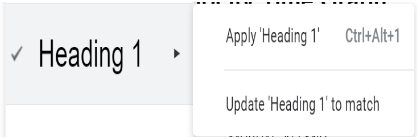
\includegraphics[width=0.8\linewidth]{2.1.png}
		\caption{Applying Heading}
	\end{figure}
	STEP 1:-As per figure we first write our heading related to our topic as mine was
	The Graphical Analysis of Velocity and displacement time graph and through
	styles we select our heading and apply Heading.
	\begin{figure}[H]
		\centering
		
\includegraphics[width=0.8\linewidth]{2.2.png}
		\caption{Justified Alignment}
	\end{figure}
	STEP 2:-As per figure now we select our written text and align all of the text through
	this desired alignment and make our text looks uniform and professional.
	
	\begin{figure}[H]
		\centering
		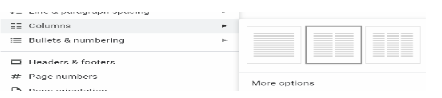
\includegraphics[width=0.8\linewidth]{2.3.png}
		\caption{Setting Up Double Column}
	\end{figure}
	STEP 3:-As per figure we select our text and apply two columns to our text.
	 
	\begin{figure}[H]
		\centering
		
\includegraphics[width=0.8\linewidth]{2.4.png}
		\caption{Bold And Italicized}
	\end{figure}
	STEP 4:-As per figure we select our text and make it bold and italic this depends on
	preference but it makes our text look professional and more easily readable for
	the reader.
	\begin{figure}[H]
		\centering
		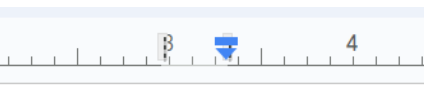
\includegraphics[width=0.8\linewidth]{2.5.png}
		\caption{Aligning With Scale}
	\end{figure}
	STEP 5:-As per Figure we play the game of the ruler and make the desired distance
	between the columns which helps us organize the columns and make it more
	appealing for the reader as a good text is one with good scaling and margins.
	\begin{figure}[H]
		\centering
		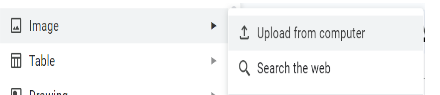
\includegraphics[width=0.8\linewidth]{2.6.png}
		\caption{Uploading Images}
	\end{figure}
	STEP 6:-As per figure we upload pictures from our computer into the text on our
	desired location.
	\begin{figure}[H]
		\centering
		
\includegraphics[width=0.8\linewidth]{2.7.png}
		\caption{Image Alignment}
	\end{figure}
	STEP 7:-As per Figure we make our image in front of the text to make it align well
	with the text so we can also name it properly along with the text.
	\begin{figure}[H]
		\centering
		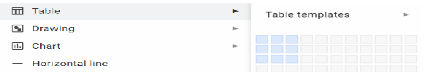
\includegraphics[width=0.8\linewidth]{2.8.png}
		\caption{Table Creation}
		\end{figure}
		STEP 8:-As per Figure 1.8 we also will be inserting 3 columns and rows into our text
		through the insert option and then by selecting column, to make a table for
		our values.
		
\end{enumerate}

\subsection{Lab Task}

\begin{itemize}
	\item Analyze existing double-column report templates for structure.
	\item Create a double-column layout using software tools like LaTeX or Word.
	\item Add sections such as Abstract, Introduction, and Results with proper headings.
	\item Insert visuals (e.g., tables or graphs) to test alignment and formatting.
\end{itemize}

\subsection{Observation}
\begin{itemize}
	\item Double-column layouts provide a compact, visually appealing structure for presenting information.
	 
	\item Software tools like LaTeX offer precise control over formatting, while Word templates provide easier customization.
	\item  Figures and tables require careful placement to ensure readability within the columns.
	\item Proper use of headings and subheadings improves the document's organization and navigation.
\end{itemize}
\subsection{Conclusion}
This experiment highlights the efficiency and professionalism of double-column layouts for scientific reporting. Tools like LaTeX and Word simplify the process, enabling users to produce high-quality, well-organized reports suitable for academic and technical dissemination.

\subsection{Question}

\begin{enumerate}
	\item What are the advantages of a double-column layout over a single-column layout?
	\item How does LaTeX differ from Microsoft Word in creating double-column reports? 
	\item What challenges might arise when placing tables or images in a double-column format?
	\item Why are double-column layouts preferred for scientific and technical documents?
	
\end{enumerate}

\newpage	

%%%%%%%%%%%%%%%%%%%%%%%%%%%%%%%%%%%%%%%%%%%%%%%%5%%%%%%%%%%%%%%%%%%%%%%%%%%%%%%%%%%%%%%%%%%%%%%%%%%%%%%%%%%%%%%%%%%%%%%%%%%%%%%%%%%%%%%%%%%%%%%%%%%%%%%%%%%%%%%%%%%%%%%%%%%%%%%%%%%%%%%%%%%%%%%%%%%%%%%%%%%%%%%%%%%%%%%%%%%%%%%%%%%%%%%%%%%%%%%%%%%%5

\begin{center}
	{\Huge \bfseries \underline{ LAB ASSESSMENT 3: Linux Basics} \par}
\end{center}
\noindent\begin{tabular}{@{}ll}
	\textbf{Lab title} :& Learning Linux Basics\\
	\textbf{Course name} :&  Introduction to Information and Communication Technology\\
	\textbf{Author name} : & Mushaf Ali Mir\\
	\textbf{Submission date} :& 12 Sept 2024 \\
\end{tabular}

\section*{Introduction}
\addcontentsline{toc}{section}{3.   \hspace{1mm}Lab Task 3}
\setcounter{section}{3}
\setcounter{figure}{0}  % Set the section counter to 2
\setcounter{subsection}{0}

Linux is a powerful and open-source operating system known for its versatility and reliability in managing software and hardware resources. Its command-line interface (CLI) is particularly valued for enabling users to execute complex tasks efficiently. This experiment focuses on learning basic Linux commands, understanding their applications, and exploring the benefits of Linux in various fields..

\subsection{Objective}
The purpose of this experiment is to familiarize users with basic Linux commands, understand their functionality, and analyze the benefits of using Linux in real-world scenarios.
\subsection{Apparatus/Materials}
\begin{enumerate}
	\item A computer or virtual machine with Linux installed (e.g., Ubuntu, Fedora)
	\item Terminal application (pre-installed in most Linux distributions).
	\item Internet connection (optional, for additional resources or command testing)
	\item Basic understanding of file systems and directory structures
	
\end{enumerate}
\subsection{Theory}
Linux, as an open-source operating system, allows users to interact with the system primarily through its CLI. Commands such as ls, cd, pwd, mkdir, rm, and chmod are fundamental for navigating and managing files and directories. Understanding these commands helps users efficiently manage resources, automate tasks, and customize system behavior. Linux’s open-source nature and robust architecture make it a preferred choice for developers, system administrators, and enthusiasts.
\subsection{Procedure}
\begin{enumerate}
	\item \textbf{Navigating Linux Files With Terminal}
	
	\begin{figure}[H]
		\centering
		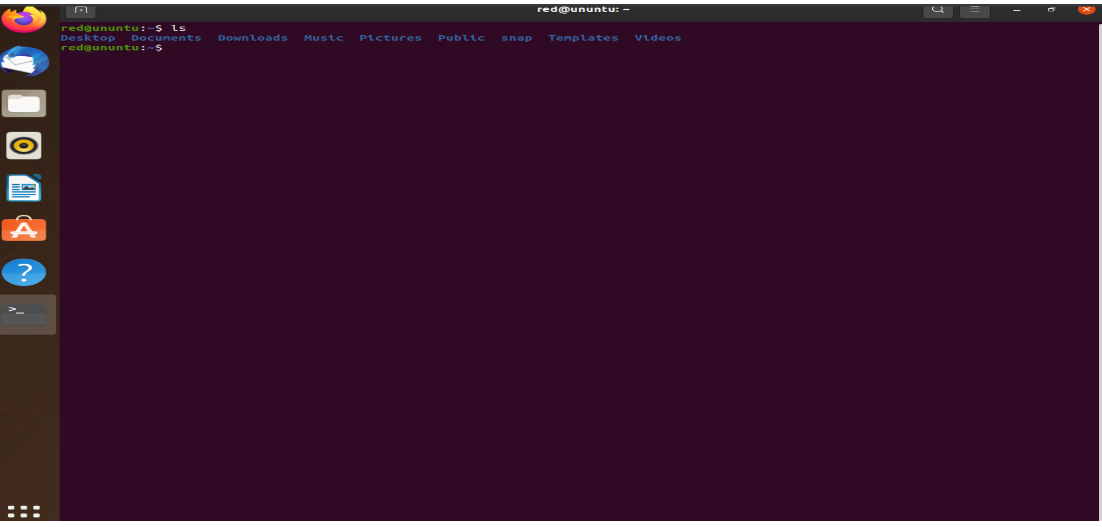
\includegraphics[width=0.8\linewidth]{3.1.png}
		\caption{-ls – List files}
	\end{figure}
	STEP 1:-We use ls to list the files and folders of the current directory,so we can find our desired folder or file
	to work with.
	\begin{figure}[H]
		\centering
		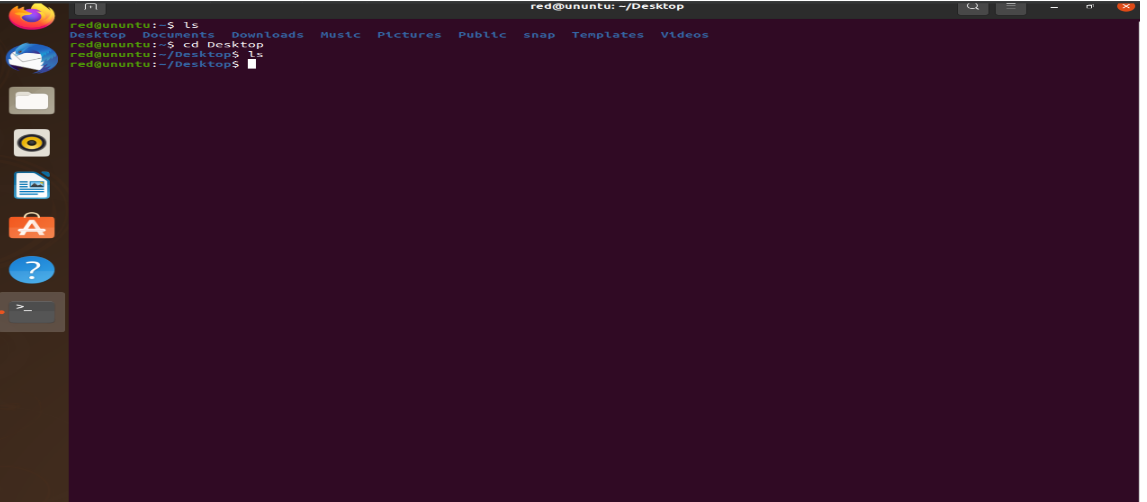
\includegraphics[width=0.8\linewidth]{3.2.png}
		\caption{-cd – Change directory:}
	\end{figure}
	STEP 2:-We use cd to change the directory from our current directory to another directory which
	is used to navigate between different folders.
	
	\begin{figure}[H]
		\centering
		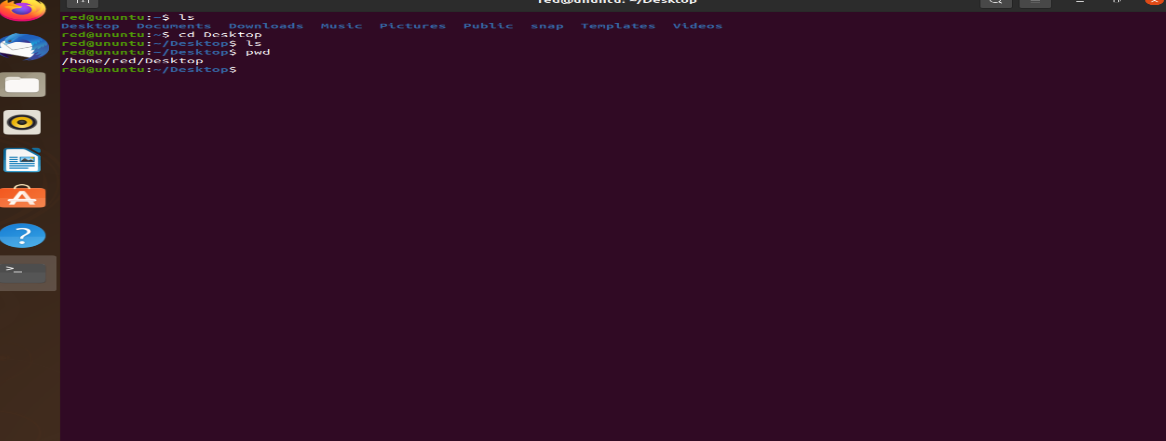
\includegraphics[width=0.8\linewidth]{3.3.png}
		\caption{-pwd – Print current working directory:}
	\end{figure}
	STEP 3:-We use pwd for printing the current directory which gives us the full location for
	our working directory and help us navigate to different directories.
	\begin{figure}[H]
		\centering
		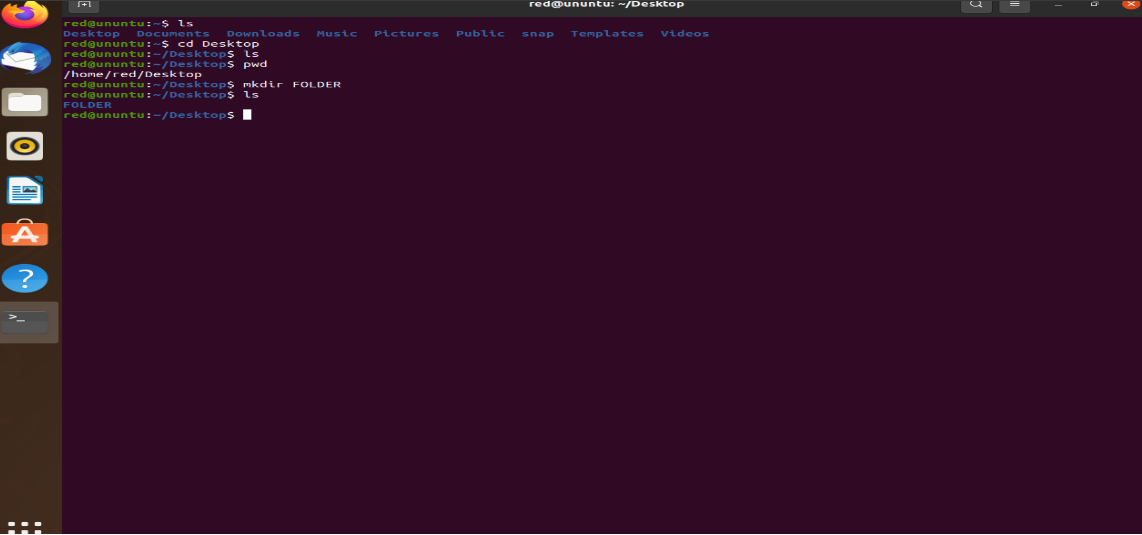
\includegraphics[width=0.8\linewidth]{3.4.png}
		\caption{-Nano – edit Text File}
	\end{figure}
	STEP 4:-We use nano to view and edit our text file and input our desired text and we can rename it.
	\begin{figure}[H]
		\centering
		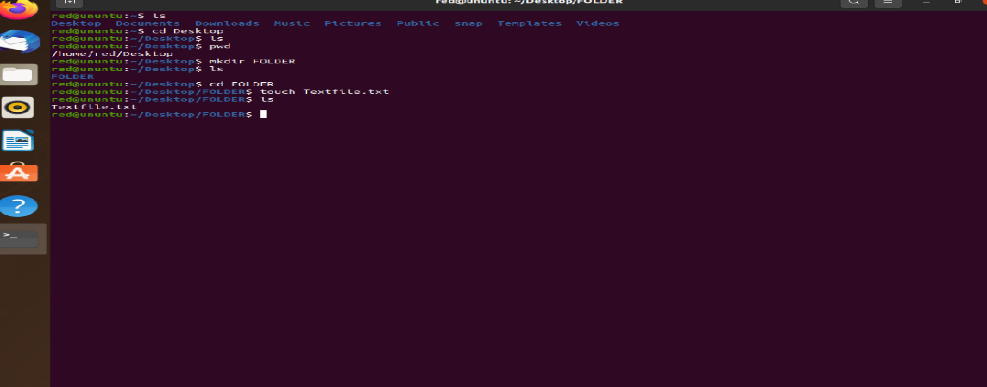
\includegraphics[width=0.8\linewidth]{3.5.png}
		\caption{-rm –To remove Files.}
	\end{figure}
	STEP 5:-We use rm to remove folders in linux and -rf for removing files this command can be
	interpreted to the Windows 10 delete option while this is CLI.
	\begin{figure}[H]
		\centering
		
\includegraphics[width=0.8\linewidth]{3.6.png}
		\caption{-cp – To copy files and directories}
	\end{figure}
	STEP 6:-We use cp to copy files or directories to different locations.we use here to move
	ICTCLASS.txt file to desktop.
	\begin{figure}[H]
		\centering
		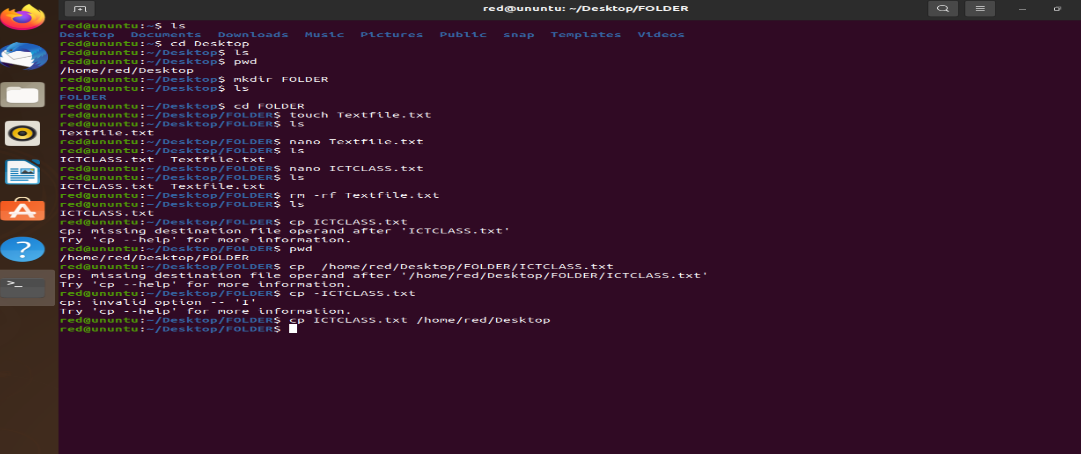
\includegraphics[width=0.8\linewidth]{3.7.png}
		\caption{-Cat – Display content Of files}
	\end{figure}
	STEP 7:-The cat command is used to display the content of files which helps us read the contents of
	our file ICTCLASS.txt..
	\begin{figure}[H]
		\centering
		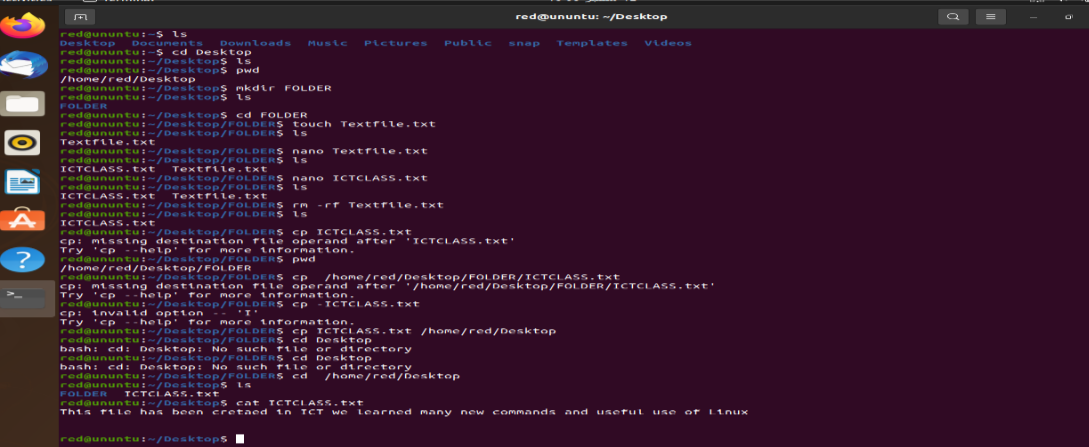
\includegraphics[width=0.8\linewidth]{3.8.png}
		\caption{-cp – Copy files or directories.}
	\end{figure}
	STEP 8:-This command is used to move or rename files in the linux terminal.
	
\end{enumerate}

\subsection{Lab Task}

\begin{itemize}
	\item Navigate through the file system using commands like cd, ls, and pwd.
	\item Create and remove directories and files using mkdir and rm.
	\item Modify file permissions using chmod and check file ownership using ls -l.
	\item Use cp and mv to copy and move files.
\end{itemize}

\subsection{Observation}
\begin{itemize}
	\item Linux commands provide a precise and efficient way to manage files and directories.
	
	\item File permissions and ownership control access to system resources, ensuring security
	\item System monitoring commands (top, df, etc.) give real-time insights into system performance.
	\item The command-line interface is faster and more flexible than graphical interfaces for repetitive tasks.
\end{itemize}
\subsection{Conclusion}
Learning Linux basics equips users with essential skills for managing files, directories, and system resources. Linux's command-line tools are powerful for performing tasks efficiently and ensuring system security. Its versatility and open-source nature make it an invaluable tool for a variety of professional and personal applications.

\subsection{Question}

\begin{enumerate}
	\item What are the benefits of using Linux over other operating systems?
	\item How does the chmod command enhance file security? 
	\item Why is understanding the file system hierarchy important in Linux?
	\item Explain the significance of top in monitoring system performance.
	
\end{enumerate}

\newpage		


%%%%%%%%%%%%%%%%%%%%%%%%%%%%%%%%%%%%%%%%%%%%%%%%5%%%%%%%%%%%%%%%%%%%%%%%%%%%%%%%%%%%%%%%%%%%%%%%%%%%%%%%%%%%%%%%%%%%%%%%%%%%%%%%%%%%%%%%%%%%%%%%%%%%%%%%%%%%%%%%%%%%%%%%%%%%%%%%%%%%%%%%%%%%%%%%%%%%%%%%%%%%%%%%%%%%%%%%%%%%%%%%%%%%%%%%%%%%%%%%%%%%5

\begin{center}
	{\Huge \bfseries \underline{ LAB ASSESSMENT 4: Slides Presentation} \par}
\end{center}
\noindent\begin{tabular}{@{}ll}
	\textbf{Lab title} :&Learning And Creating Excel Slides \\
	\textbf{Course name} :&  Introduction to Information and Communication Technology\\
	\textbf{Author name} : & Mushaf Ali Mir\\
	\textbf{Submission date} :& 18 Oct 2024 \\
\end{tabular}

\section*{Introduction}
\addcontentsline{toc}{section}{4.   \hspace{1mm}Lab Task 4}
\setcounter{section}{4}
\setcounter{figure}{0}  % Set the section counter to 2
\setcounter{subsection}{0}

Creating effective presentations is an essential skill in both academic and professional settings. This experiment focuses on learning the basics of crafting visually appealing presentations, including inserting multimedia elements such as images, audio, and videos, and utilizing professional templates to enhance communication and engagement. By mastering these techniques, users can deliver impactful presentations tailored to their audience.

\subsection{Objective}
The purpose of this experiment is to develop skills in creating visually appealing and engaging presentations by learning to insert multimedia elements, use professional templates, and apply design principles.
\subsection{Apparatus/Materials}
\begin{enumerate}
	\item Presentation software (e.g., Microsoft PowerPoint, Google Slides, Canva, or Prezi)
	\item Access to multimedia resources (images, audio, and video files).
	\item IInternet connection (for downloading templates or assets)
	\item Computer with basic input devices (mouse, keyboard)
	
\end{enumerate}
\subsection{Theory}
A good presentation is not just about content but also about how the content is visually and audibly communicated. Multimedia elements like images, videos, and audio enhance engagement and help convey complex ideas effectively. Templates provide a structured and professional design framework, saving time while maintaining visual appeal. Theories of visual hierarchy, minimalism, and consistency guide effective presentation design.
\subsection{Procedure}
\begin{enumerate}
	\item \textbf{Creating Slides Presentation}
	
	\begin{figure}[H]
		\centering
		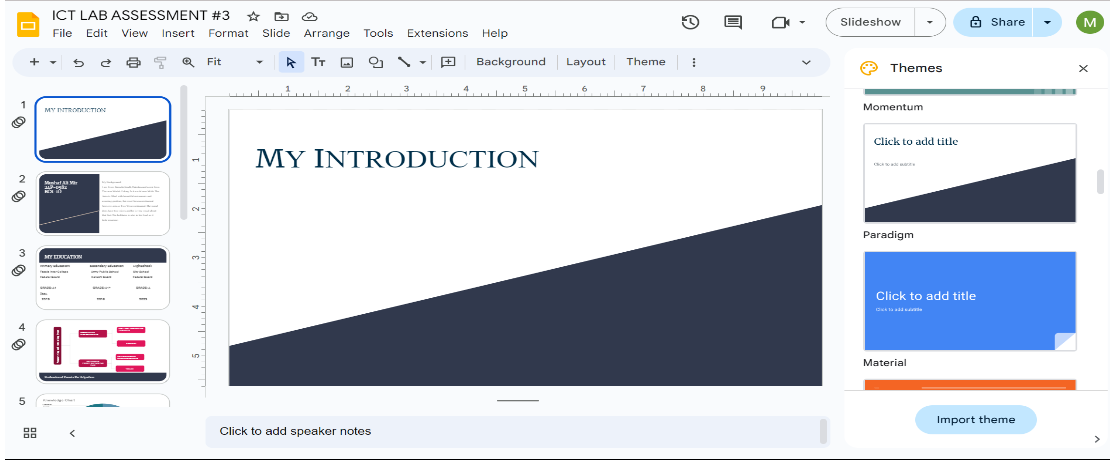
\includegraphics[width=0.8\linewidth]{4.1.png}
		\caption{Theme Selection}
	\end{figure}
	STEP 1:-Selecting your prefered Theme from the them selection.I selected “paradigm”.
	\begin{figure}[H]
		\centering
		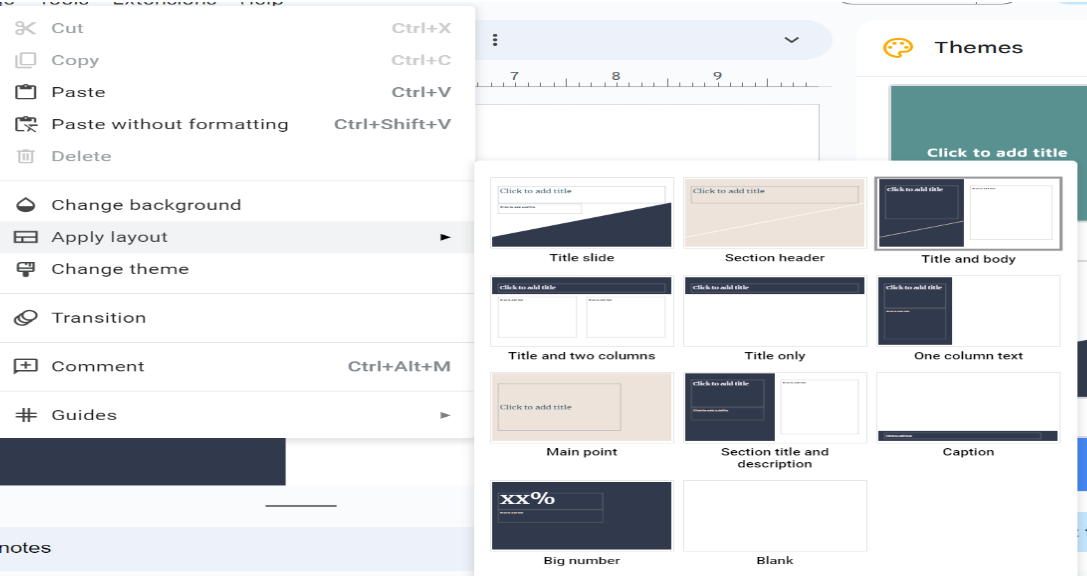
\includegraphics[width=0.8\linewidth]{4.2.png}
		\caption{Layout Selection}
	\end{figure}
	STEP 2:-Select your desired layout by right click and going to layout tab and select the
	most appealing i selected “title and body”.
	
	\begin{figure}[H]
		\centering
		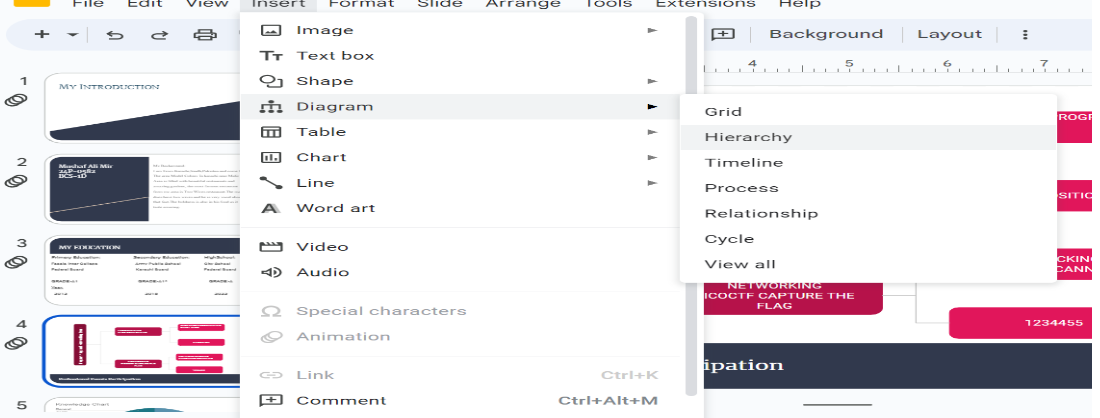
\includegraphics[width=0.8\linewidth]{4.3.png}
		\caption{Hierarchy Diagram}
	\end{figure}
	STEP 3:-Select Your preferred Hierarchy diagram to meet your need.
	\begin{figure}[H]
		\centering
		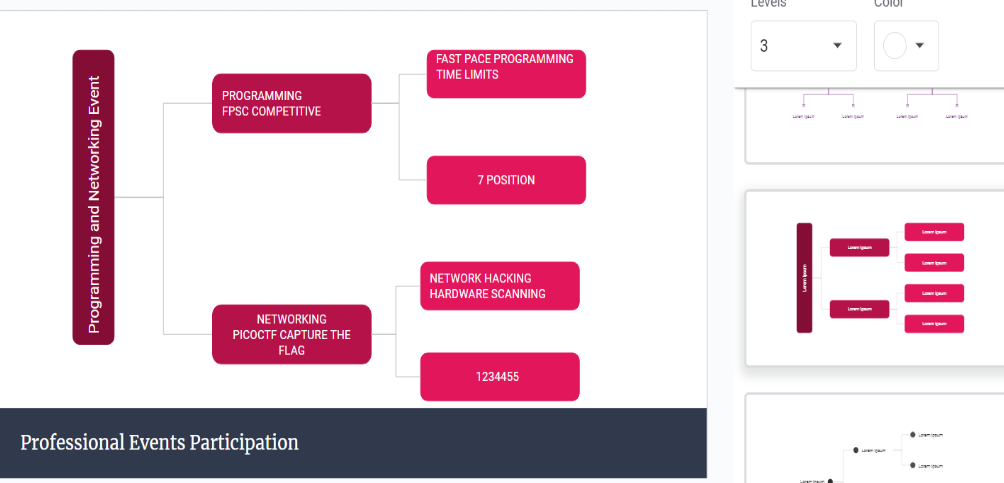
\includegraphics[width=0.8\linewidth]{4.4.png}
		\caption{Diagram Selection}
	\end{figure}
	STEP 4:-Select Your preferred Hierarchy diagram to meet your need.
	\begin{figure}[H]
		\centering
		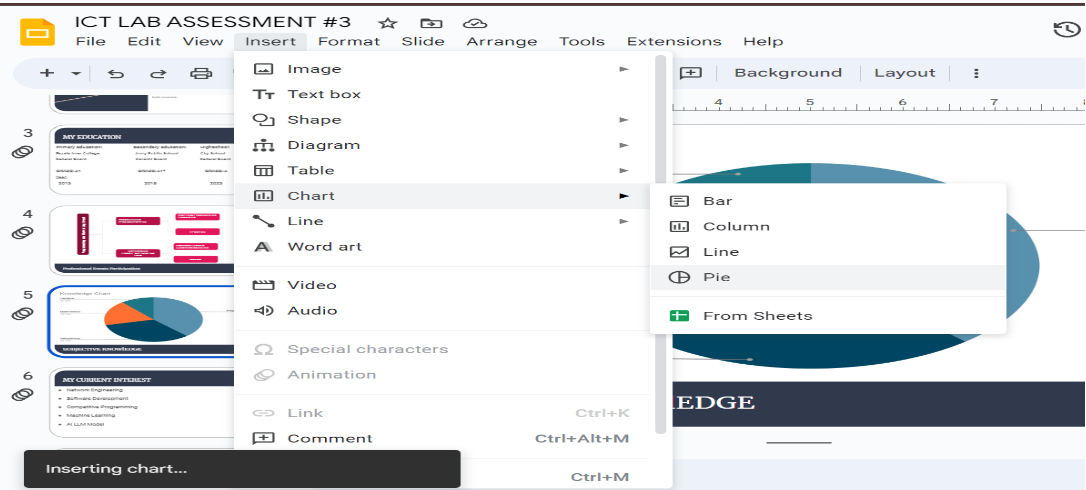
\includegraphics[width=0.8\linewidth]{4.5.png}
		\caption{Pie Chart Selection}
	\end{figure}
	STEP 5:-Select the best pie chat to display information here i used pie chart to display
	my knowledge.
	\begin{figure}[H]
		\centering
		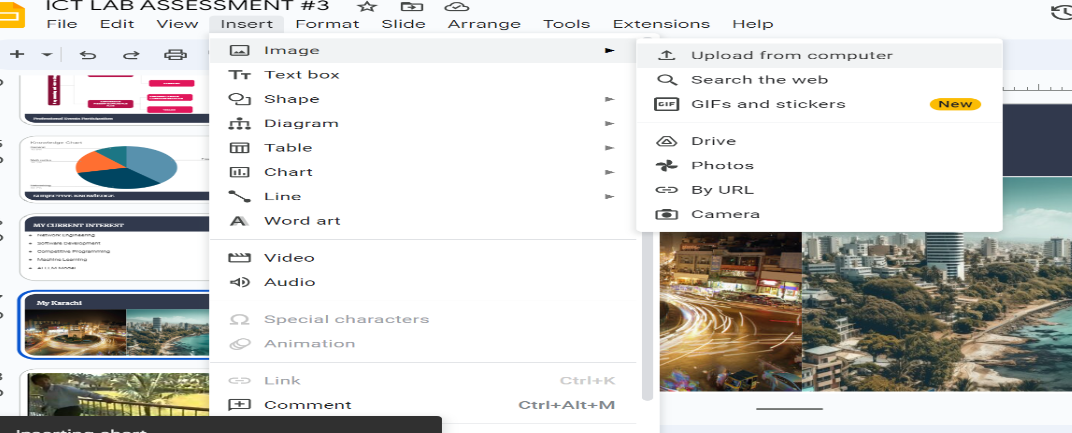
\includegraphics[width=0.8\linewidth]{4.6.png}
		\caption{Uploading Image}
	\end{figure}
	STEP 6:-Upload your desired image into the presentation i used my karachi city image to
	display its beauty.
	\begin{figure}[H]
		\centering
		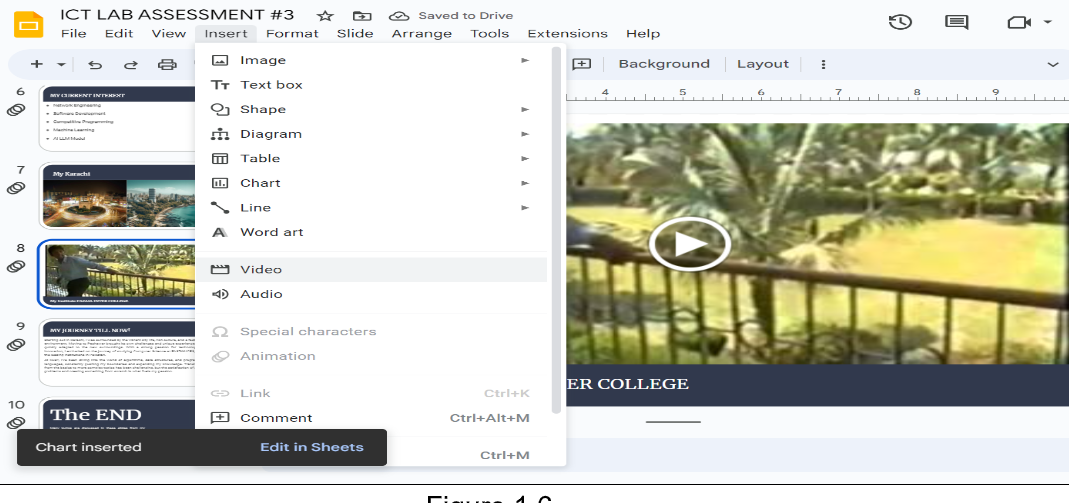
\includegraphics[width=0.8\linewidth]{4.7.png}
		\caption{Uploading Video}
	\end{figure}
	STEP 7:-Insert your desired image onto presentation from insert tab and choosing a link
	for video..
	\begin{figure}[H]
		\centering
		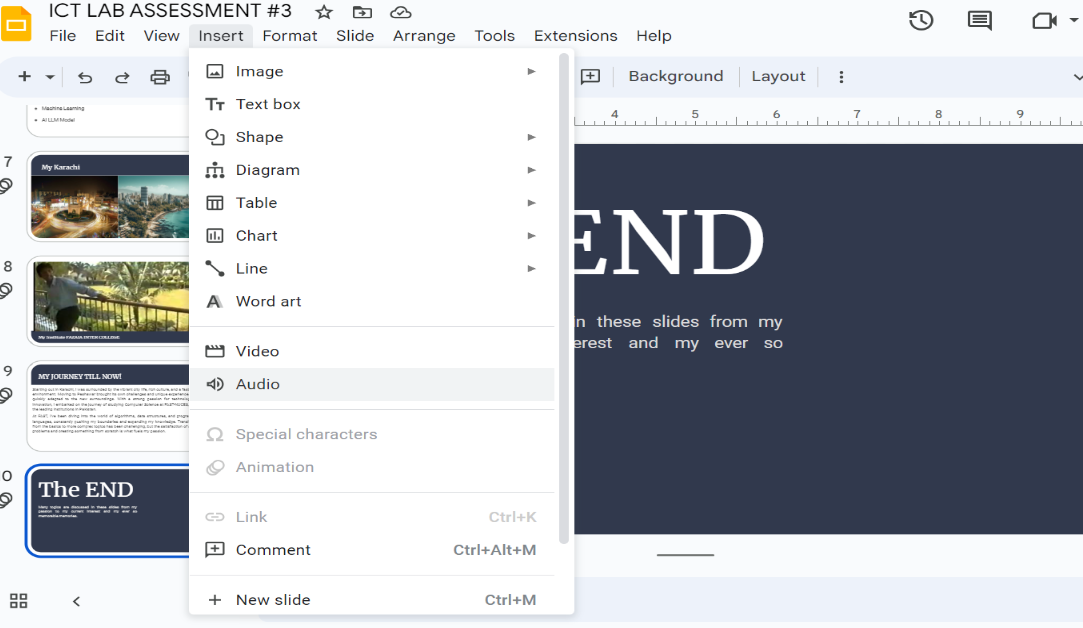
\includegraphics[width=0.8\linewidth]{4.8.png}
		\caption{Uploading Audio}
	\end{figure}
	STEP 8:-Insert any audio in your presentation from insert tab and make your
	presentation more appealing.
	
\end{enumerate}

\subsection{Lab Task}

\begin{itemize}
	\item Insert and format images within slides to support key points.
	\item Add and configure audio files for background music or narration.
	\item Embed and play video clips relevant to the presentation topic.
	\item Experiment with different slide templates and themes for a cohesive design.
\end{itemize}

\subsection{Observation}
\begin{itemize}
	\item High-quality templates significantly improve the visual appeal of a presentation.
	
	
	\item Images and videos help clarify and emphasize key points, increasing audience engagement.
	\item Overuse of animations and transitions can distract viewers from the main content..
	\item Adding multimedia requires attention to file compatibility and proper formatting.
\end{itemize}
\subsection{Conclusion}
Learning to create presentations with multimedia elements and professional templates enhances the ability to communicate ideas effectively. A well-designed presentation can capture and hold the audience's attention while delivering content in an organized and engaging manner. Mastering these techniques equips users with the tools to present confidently in various contexts.

\subsection{Question}

\begin{enumerate}
	\item How do templates improve the efficiency of creating presentations?
	
	\item What are the benefits of embedding videos in a presentation? 
	\item Explain the importance of consistency in font styles and color schemes.
	\item What factors should be considered when choosing multimedia elements for a presentation?
	
\end{enumerate}

\newpage

%%%%%%%%%%%%%%%%%%%%%%%%%%%%%%%%%%%%%%%%%%%%%%%%5%%%%%%%%%%%%%%%%%%%%%%%%%%%%%%%%%%%%%%%%%%%%%%%%%%%%%%%%%%%%%%%%%%%%%%%%%%%%%%%%%%%%%%%%%%%%%%%%%%%%%%%%%%%%%%%%%%%%%%%%%%%%%%%%%%%%%%%%%%%%%%%%%%%%%%%%%%%%%%%%%%%%%%%%%%%%%%%%%%%%%%%%%%%%%%%%%%%5

\begin{center}
	{\Huge \bfseries \underline{ LAB ASSESSMENT 5: Creating Google Sheets } \par}
\end{center}
\noindent\begin{tabular}{@{}ll}
	\textbf{Lab title} :&Learning And Creating Google Sheets \\
	\textbf{Course name} :&  Introduction to Information and Communication Technology\\
	\textbf{Author name} : & Mushaf Ali Mir\\
	\textbf{Submission date} :& 7 Nov 2024 \\
\end{tabular}

\section*{Introduction}
\addcontentsline{toc}{section}{5.   \hspace{1mm}Lab Task 5}
\setcounter{section}{5}
\setcounter{figure}{0}  % Set the section counter to 2
\setcounter{subsection}{0}

Spreadsheet applications are essential tools for managing and analyzing data efficiently. This experiment focuses on creating and editing spreadsheets, adding charts and diagrams for data visualization, and applying formatting techniques to enhance clarity and presentation. These skills are widely applicable across academic, professional, and personal tasks.

\subsection{Objective}
The purpose of this experiment is to learn how to create, format, and edit spreadsheets, use formulas for data analysis, and incorporate charts and diagrams to effectively visualize data.

\subsection{Apparatus/Materials}
\begin{enumerate}
	\item A spreadsheet application (e.g., Microsoft Excel, Google Sheets, LibreOffice Calc)
	\item Sample data set (e.g., sales, survey results, or attendance records)
	\item Basic understanding of spreadsheet navigation and structure
	\item Computer or mobile device
	
\end{enumerate}
\subsection{Theory}
Spreadsheet applications organize data in rows and columns, offering powerful tools for analysis and visualization. Charts, such as bar graphs, line graphs, and pie charts, highlight trends and patterns within the data, while diagrams add clarity and structure. Using formulas and functions like SUM, AVERAGE, and IF enables efficient data processing. Formatting tools improve readability and aesthetics, making the spreadsheet more user-friendly and professional.

\subsection{Procedure}
\begin{enumerate}
	\item \textbf{Creating Slides Presentation}
	
	\begin{figure}[H]
		\centering
		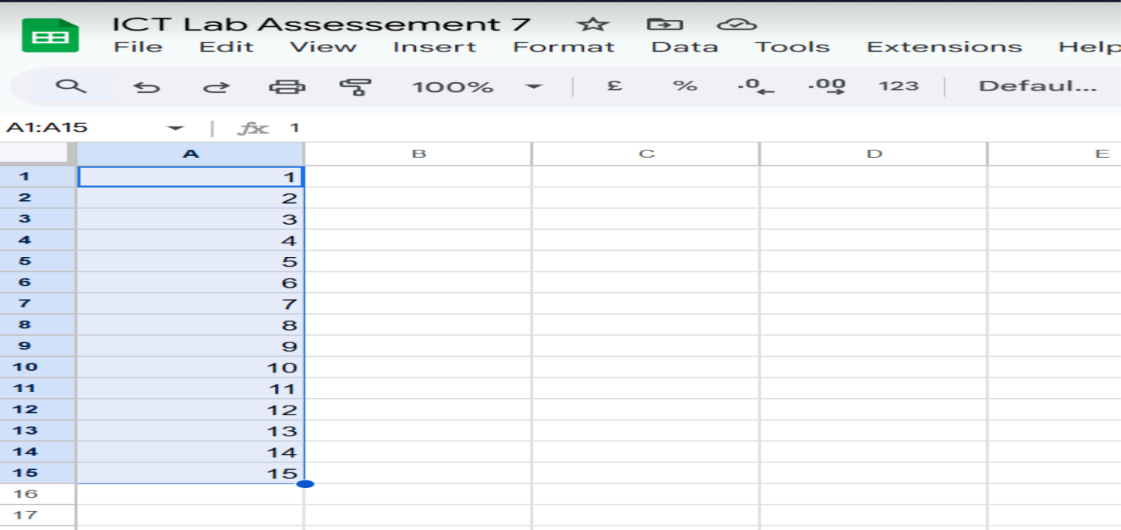
\includegraphics[width=0.8\linewidth]{5.1.png}
		\caption{Row Expanding }
	\end{figure}
	STEP 1:-Expanding rows by dragging.
	\begin{figure}[H]
		\centering
		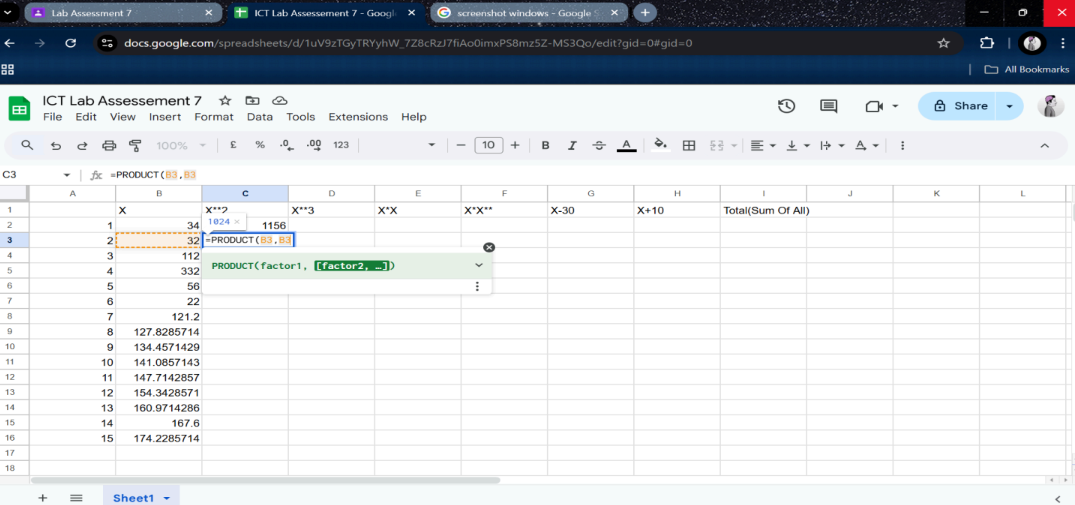
\includegraphics[width=0.8\linewidth]{5.2.png}
		\caption{Product Formula}
	\end{figure}
	STEP 2:-Applying Product Function.
	
	\begin{figure}[H]
		\centering
		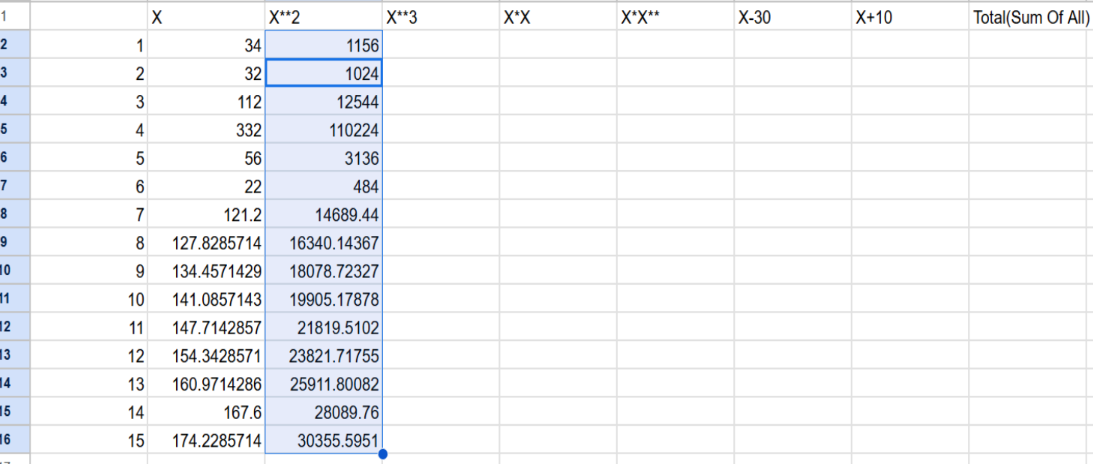
\includegraphics[width=0.8\linewidth]{5.3.png}
		\caption{Square Function}
	\end{figure}
	STEP 3:-Square Function and expanding the column. diagram to meet your need.
	\begin{figure}[H]
		\centering
		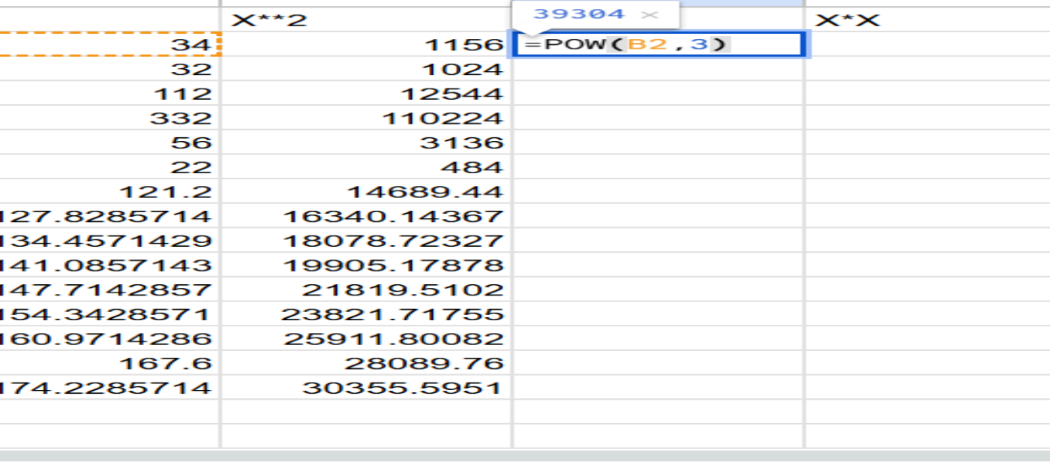
\includegraphics[width=0.8\linewidth]{5.4.png}
		\caption{Pow Function}
	\end{figure}
	STEP 4:-Using Pow function For the Cube.
	\begin{figure}[H]
		\centering
		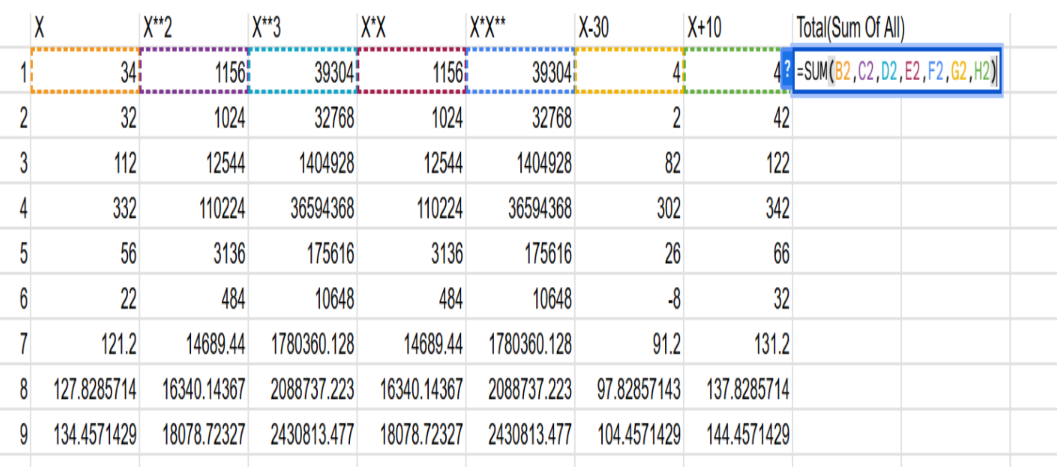
\includegraphics[width=0.8\linewidth]{5.7.png}
		\caption{Sum Function}
	\end{figure}
	STEP 5:-Using the Sum function to Sum all the entities of the row.
	my knowledge.
	\begin{figure}[H]
		\centering
		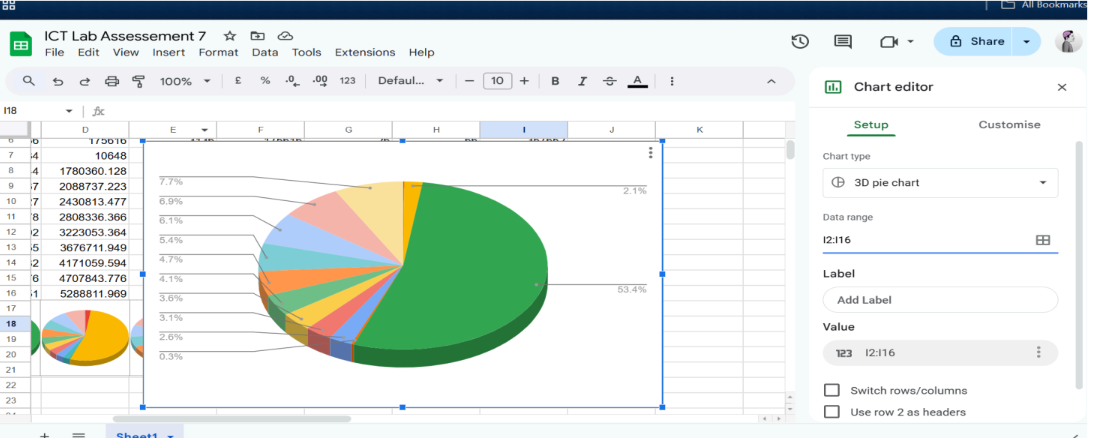
\includegraphics[width=0.8\linewidth]{5.6.png}
		\caption{Pie Chart}
	\end{figure}
	STEP 6:-Inserting Pie Chart And Graph for overall comparison.
	\begin{figure}[H]
		\centering
		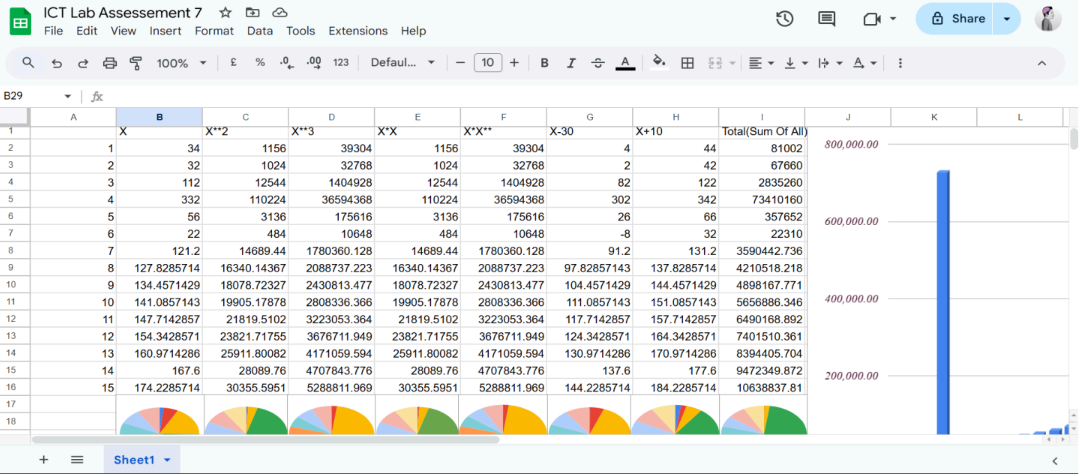
\includegraphics[width=0.8\linewidth]{5.5.png}
		\caption{Sheet Ready}
	\end{figure}
	STEP 7:-The Final Result.
	
\end{enumerate}

\subsection{Lab Task}

\begin{itemize}
	\item Input and organize sample data into a spreadsheet.
	\item Create and customize charts (e.g., bar, line, and pie charts) to represent data visually.
	\item Insert diagrams to structure information clearly.
	\item Apply formatting to improve presentation, such as conditional formatting, borders, and cell shading..
\end{itemize}

\subsection{Observation}
\begin{itemize}
	\item Spreadsheets provide a structured way to manage and analyze large datasets.
	
	
	\item Charts and diagrams effectively communicate trends and relationships in the data.
	\item Using formulas saves time and ensures accuracy in calculations.
	\item Proper formatting enhances data readability and professionalism.
\end{itemize}
\subsection{Conclusion}
Learning to create and edit spreadsheets is a fundamental skill for data management and visualization. By using charts, diagrams, and formulas, users can analyze and present data effectively. These tools are indispensable in various fields, including finance, education, and research.

\subsection{Question}

\begin{enumerate}
	\item What are the benefits of using charts to represent data in a spreadsheet?
	
	\item How do formulas improve efficiency when working with large datasets?
	\item Explain the role of conditional formatting in spreadsheet presentation.
	\item What is the difference between bar charts and pie charts in data visualization?
	?
	
\end{enumerate}

\newpage

%%%%%%%%%%%%%%%%%%%%%%%%%%%%%%%%%%%%%%%%%%%%%%%%5%%%%%%%%%%%%%%%%%%%%%%%%%%%%%%%%%%%%%%%%%%%%%%%%%%%%%%%%%%%%%%%%%%%%%%%%%%%%%%%%%%%%%%%%%%%%%%%%%%%%%%%%%%%%%%%%%%%%%%%%%%%%%%%%%%%%%%%%%%%%%%%%%%%%%%%%%%%%%%%%%%%%%%%%%%%%%%%%%%%%%%%%%%%%%%%%%%%5

\begin{center}
	{\Huge \bfseries \underline{ LAB ASSESSMENT 6: Creating LAN } \par}
\end{center}
\noindent\begin{tabular}{@{}ll}
	\textbf{Lab title} :&Learning And Creating Local Area Network \\
	\textbf{Course name} :&  Introduction to Information and Communication Technology\\
	\textbf{Author name} : & Mushaf Ali Mir\\
	\textbf{Submission date} :& 16 Nov 2024 \\
\end{tabular}

\section*{Introduction}
\addcontentsline{toc}{section}{6.   \hspace{1mm}Lab Task 6}
\setcounter{section}{6}
\setcounter{figure}{0}  % Set the section counter to 2
\setcounter{subsection}{0}

A Local Area Network (LAN) is a network of computers and devices interconnected within a limited area such as an office, building, or campus. Setting up a LAN involves configuring various hardware components, network devices, and ensuring smooth communication between devices. This experiment focuses on understanding the fundamentals of creating a LAN, including hardware setup, IP addressing, and configuring network devices to enable communication.

\subsection{Objective}
The purpose of this experiment is to design and implement a Local Area Network (LAN), configure network devices, and understand the key components required for effective communication within the network.

\subsection{Apparatus/Materials}
\begin{enumerate}
	\item Computers or Devices (PCs, laptops, or workstations) LibreOffice Calc)
	\item Network Interface Cards (NICs)
	\item Operating System (e.g., Windows, Linux) with network configuration tools
	\item IP addressing scheme (static or dynamic IP addresses)
	
\end{enumerate}
\subsection{Theory}
A Local Area Network (LAN) allows devices to communicate within a limited geographic area. The basic components of a LAN include routers, switches, and network cables that enable data transmission between devices. The LAN may use either static or dynamic IP addressing, with the latter relying on a DHCP server to assign IP addresses automatically. By establishing a LAN, devices within the network can share resources like files, printers, and internet connections.

\subsection{Procedure}
\begin{enumerate}
	\item \textbf{Creating Slides Presentation}
	
	\begin{figure}[H]
		\centering
		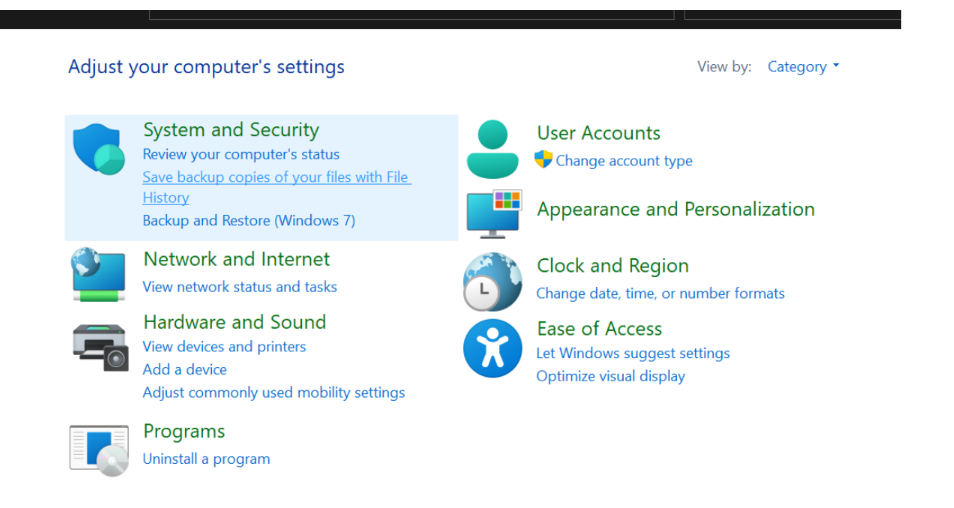
\includegraphics[width=0.8\linewidth]{6.1.png}
		\caption{Lan Setup }
	\end{figure}
	STEP 1:-We Setup our lan for 2 windows devices first we connect both of them to save network in our case to my mobile
	network hotspot and then properly set their setting like in the following steps.After successful connection go to our control panel setting and there we select network and internet settings.
	\begin{figure}[H]
		\centering
		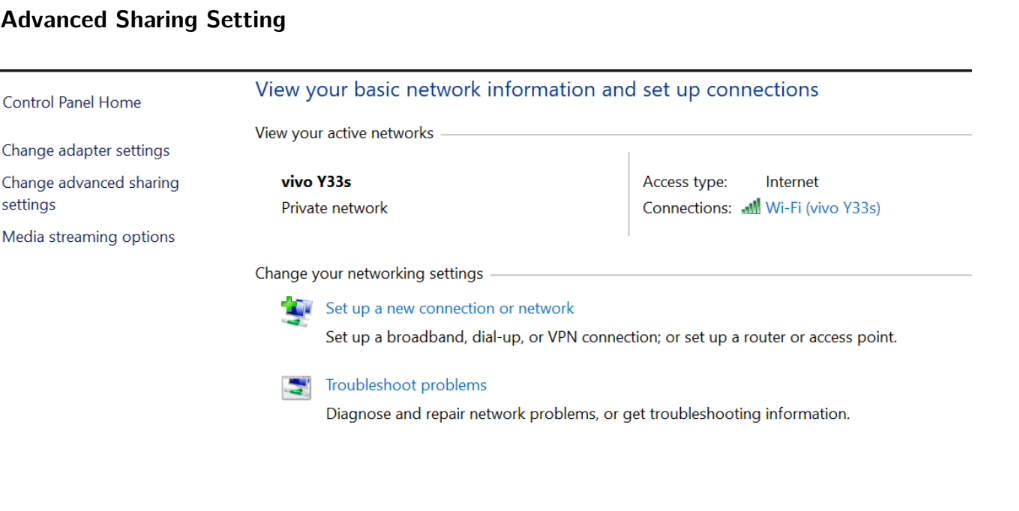
\includegraphics[width=0.8\linewidth]{6.2.png}
		\caption{Advanced Sharing}
	\end{figure}
	STEP 2:-After Selecting network setting in our control panel we select advanced sharing setting in our left in the 3rd
	option.
	
	\begin{figure}[H]
		\centering
		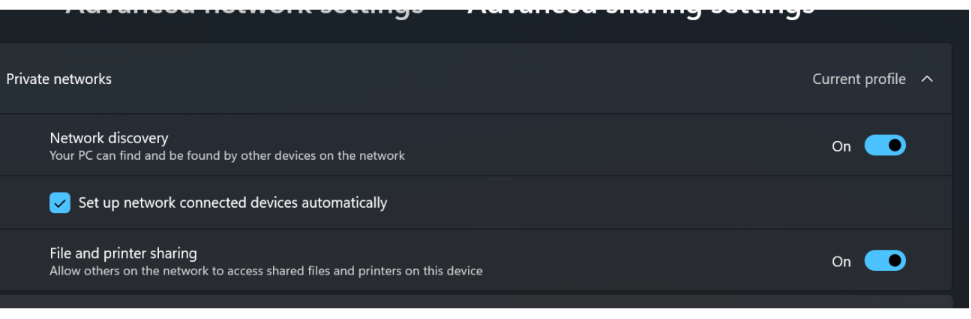
\includegraphics[width=0.8\linewidth]{6.3.png}
		\caption{Enable File Sharing}
	\end{figure}
	STEP 3:-In our advanced sharing option we select Our current profile setting and select the network discovery option and
	file sharing so we can share the files the other device on the lan must also enable these option for communication
	and data transfer.
	\begin{figure}[H]
		\centering
		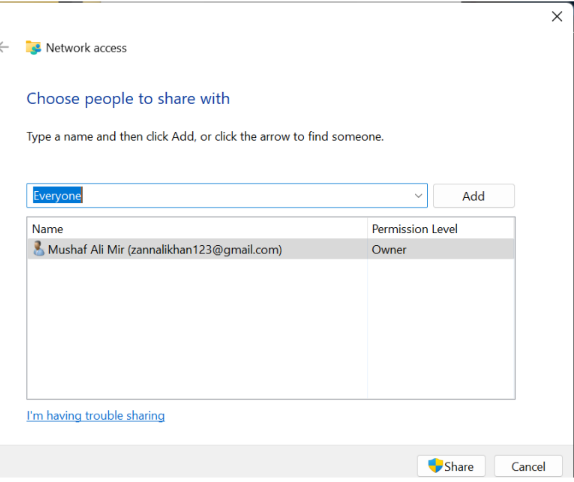
\includegraphics[width=0.8\linewidth]{6.5.png}
		\caption{File Permission}
	\end{figure}
	STEP 4:-After enabling the setting we can share our files through the file or folder setting and going to the sharing
	section and selecting share to share our file or folder in our case we select everyone to share our file with everyone
	on the network on the network access setting in Fig [5] as it a privately owned and governed network we do not
	have unwanted access and use.
	\begin{figure}[H]
		\centering
		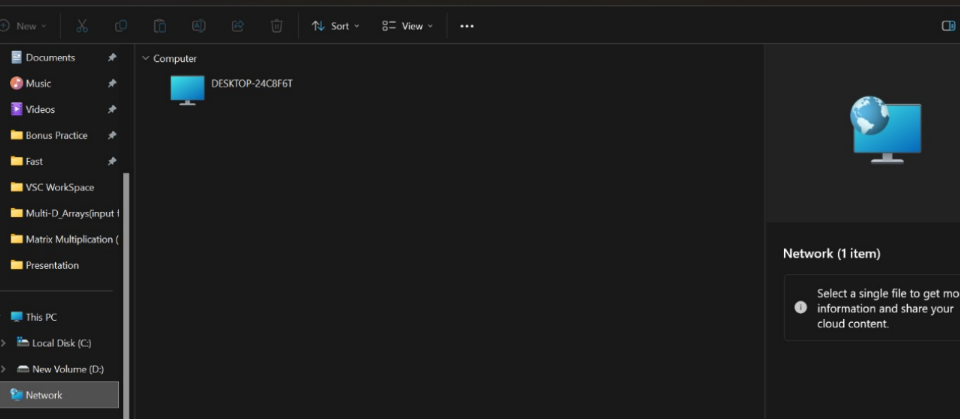
\includegraphics[width=0.8\linewidth]{6.6.png}
		\caption{Access Device}
	\end{figure}
	STEP 5:-I access my device through the Network option in my pc.
	my knowledge.
	\begin{figure}[H]
		\centering
		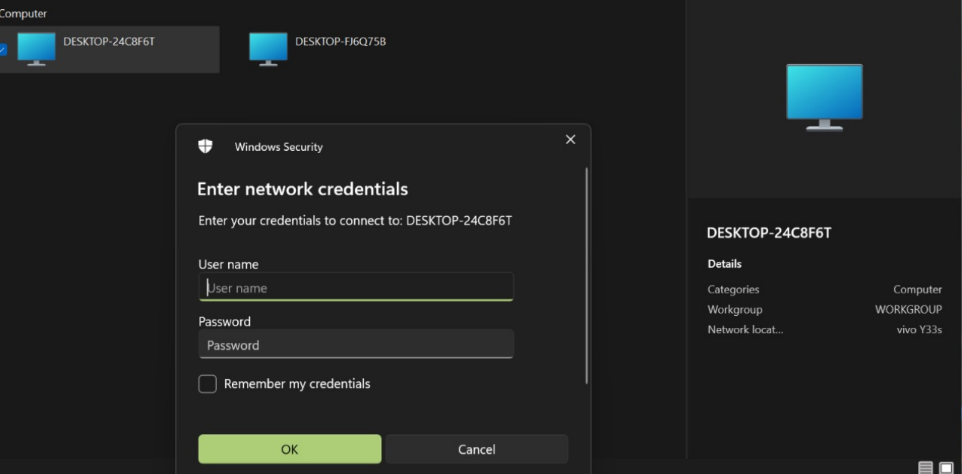
\includegraphics[width=0.8\linewidth]{6.7.png}
		\caption{Network Credentials }
	\end{figure}
	STEP 6:-To make our lan safe for demonstration sake we require a username and password for access to our pc on the
	second computer.
	\begin{figure}[H]
		\centering
		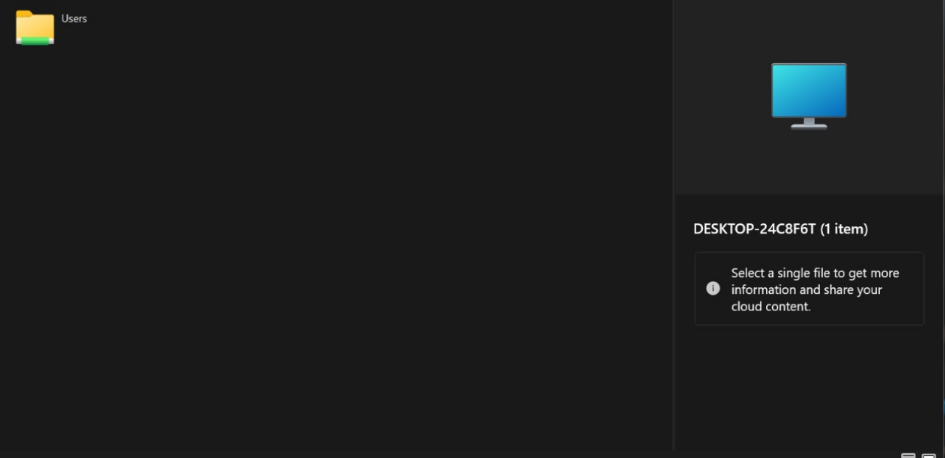
\includegraphics[width=0.8\linewidth]{6.8.png}
		\caption{Accessing Files}
	\end{figure}
	STEP 7:-After successful access to the device we access our desired files for our use.The file should have share permission.
	
\end{enumerate}

\subsection{Lab Task}

\begin{itemize}
	\item Assign static or dynamic IP addresses to devices using the network configuration settings.
	\item Test network connectivity between devices using tools like ping.
	\item Configure file and printer sharing to enable resource sharing across the network.
	
	\item Connect multiple devices using Ethernet cables to the router or switch.
\end{itemize}

\subsection{Observation}
\begin{itemize}
	\item Devices on the LAN are successfully able to communicate with each other after configuration.
	
	
	\item The router or switch manages the flow of data between devices.
	\item Resource sharing (files and printers) becomes functional after configuring the necessary settings.
	\item The choice of static or dynamic IP addressing influences network management and device communication.
\end{itemize}
\subsection{Conclusion}
Setting up a Local Area Network (LAN) provides a solid foundation for managing communication and resource sharing between multiple devices within a confined area. Understanding LAN architecture and configuring network devices is essential for enabling smooth, reliable network performance. This experiment demonstrates the importance of proper network design and device configuration for optimal functionality.

\subsection{Question}

\begin{enumerate}
	\item What are the advantages of using a switch instead of a hub in a LAN setup?
	
	\item How does DHCP simplify IP address management in a LAN?
	\item How do static IP addresses differ from dynamic IP addresses in a network setup?
	\item What security measures should be taken when setting up a LAN to protect sensitive data?
	
\end{enumerate}

\newpage
	
%%%%%%%%%%%%%%%%%%%%%%%%%%%%%%%%%%%%%%%%%%%%%%%%5%%%%%%%%%%%%%%%%%%%%%%%%%%%%%%%%%%%%%%%%%%%%%%%%%%%%%%%%%%%%%%%%%%%%%%%%%%%%%%%%%%%%%%%%%%%%%%%%%%%%%%%%%%%%%%%%%%%%%%%%%%%%%%%%%%%%%%%%%%%%%%%%%%%%%%%%%%%%%%%%%%%%%%%%%%%%%%%%%%%%%%%%%%%%%%%%%%%5

\begin{center}
	{\Huge \bfseries \underline{ LAB ASSESSMENT 7: Number System} \par}
\end{center}
\noindent\begin{tabular}{@{}ll}
	\textbf{Lab title} :&Learning And Creating Google Sheets \\
	\textbf{Course name} :&  Introduction to Information and Communication Technology\\
	\textbf{Author name} : & Mushaf Ali Mir\\
	\textbf{Submission date} :& 16 Nov 2024 \\
\end{tabular}

\section*{Introduction}
\addcontentsline{toc}{section}{7.   \hspace{1mm}Lab Task 7}
\setcounter{section}{7}
\setcounter{figure}{0}  % Set the section counter to 2
\setcounter{subsection}{0}

The number system forms the foundation of digital computing and mathematics, involving different bases such as binary (base 2), decimal (base 10), octal (base 8), and hexadecimal (base 16). Understanding the conversion between these systems is crucial for various applications in computing, digital logic design, and data representation. This experiment focuses on converting numbers between different systems, such as decimal to binary, binary to decimal, and others, while understanding the principles behind these conversions.

\subsection{Objective}
The purpose of this experiment is to understand the number systems used in computing and to perform conversions between different number systems, such as decimal, binary, octal, and hexadecimal.

\subsection{Apparatus/Materials}
\begin{enumerate}
	\item Calculator (optional)
	\item Spreadsheet application (optional, for automated calculations)
	\item Pen and paper (for manual calculations
	\item Computer or reference material for number system tables
	
\end{enumerate}
\subsection{Theory}
Spreadsheet applications organize data in Number systems represent numerical values using different bases:

Decimal (Base 10): Uses digits 0–9; most commonly used in everyday arithmetic.
Binary (Base 2): Uses digits 0 and 1; fundamental in computing and digital systems.
Octal (Base 8): Uses digits 0–7; often used in digital electronics.
Hexadecimal (Base 16): Uses digits 0–9 and letters A–F; widely used in programming and memory addressing.
Conversions between these systems rely on positional value and arithmetic rules. For example, to convert a decimal number to binary, divide the number repeatedly by 2, recording the remainders.

\subsection{Types Of Number System}

There are mainly four types of the number system in computer. Binary Number System: The binary
number system is the most fundamental number system used in computer science. It uses only two digits,
0 and 1, to represent all numbers and data. Decimal Number System: The decimal number system is also
used in computer science, but it is not as fundamental as the binary system. It uses ten digits, 0 through 9, to
represent numbers. Octal Number System: The octal number system uses eight digits, 0 through 7, to represent
numbers. It is commonly used in computer programming and digital electronics. Hexadecimal Number System:
The hexadecimal number system uses 16 digits, including 0 through 9 and A through F, to represent numbers.
It is often used in computer programming and digital electronics.

\subsection{Procedure}
\begin{enumerate}
	\item \textbf{Binary Conversions}
	
	To convert a decimal number to binary, we divide the decimal number by 2 repeatedly and write the remainder
	in reverse order.
	158 / 2 = 79 remainder 0 79 / 2 = 39 remainder 1 39 / 2 = 19 remainder 1 19 / 2 = 9 remainder 1 9 / 2 =
	4 remainder 1 4 / 2 = 2 remainder 0 2 / 2 = 1 remainder 0 1 / 2 = 0 remainder 1
	Therefore, the binary equivalent of 158 is 10011110.
	
	\item \textbf{Octal Conversion}
	
	To convert a decimal number to an octal, we divide the decimal number by 8 repeatedly and write the remainder
	in reverse order.
	158 / 8 = 19 remainder 6 19 / 8 = 2 remainder 3 2 / 8 = 0 remainder 2
	Therefore, the octal equivalent of 158 is 236
	
	\item \textbf{Hexadecimal Conversion}
	
	To convert a decimal number to hexadecimal, we divide the decimal number by 16 repeatedly and write the
	remainder in reverse order. For remainders greater than 9, we use letters A-F.
	158 / 16 = 9 remainder 14 (E) 9 / 16 = 0 remainder 9
	Therefore, the hexadecimal equivalent of 158 is 9E
	
	
\end{enumerate}

\subsection{Lab Task}

\begin{itemize}
	\item Convert a decimal number to binary, octal, and hexadecimal.
	\item Convert a binary number to decimal, octal, and hexadecimal
	\item Verify conversions using reverse operations (e.g., binary to decimal and back)
	\item Perform manual calculations for practice and compare results with automated tools.
\end{itemize}

\subsection{Observation}
\begin{itemize}
	\item Decimal numbers can be successfully converted to binary by repeated division by 2.
	
	
	\item Binary numbers are converted to decimal using positional values and powers of 2.
	\item Hexadecimal values simplify representation of large binary numbers due to their compactness.
	\item Each number system has specific use cases, such as binary for machine language and hexadecimal for memory addressing.
\end{itemize}
\subsection{Conclusion}
Understanding number systems and their conversions is fundamental to computing and digital electronics. Mastering these conversions enables effective communication between humans and machines. This experiment highlights the methods and importance of number system conversions in various technical fields.

\subsection{Question}

\begin{enumerate}
	\item How does the binary system represent numbers differently from the decimal system?
	
	\item Why is the hexadecimal system preferred in memory addressing?
	\item Explain the step-by-step process for converting a decimal number to binary.
	\item How is the octal system related to binary, and why is it used in digital systems?
	
\end{enumerate}

\newpage


%%%%%%%%%%%%%%%%%%%%%%%%%%%%%%%%%%%%%%%%%%%%%%%%5%%%%%%%%%%%%%%%%%%%%%%%%%%%%%%%%%%%%%%%%%%%%%%%%%%%%%%%%%%%%%%%%%%%%%%%%%%%%%%%%%%%%%%%%%%%%%%%%%%%%%%%%%%%%%%%%%%%%%%%%%%%%%%%%%%%%%%%%%%%%%%%%%%%%%%%%%%%%%%%%%%%%%%%%%%%%%%%%%%%%%%%%%%%%%%%%%%%5

\begin{center}
	{\Huge \bfseries \underline{ LAB ASSESSMENT 8: Html Development } \par}
\end{center}
\noindent\begin{tabular}{@{}ll}
	\textbf{Lab title} :&Learning And Creating HTML Web Pages \\
	\textbf{Course name} :&  Introduction to Information and Communication Technology\\
	\textbf{Author name} : & Mushaf Ali Mir\\
	\textbf{Submission date} :& 27 Nov 2024 \\
\end{tabular}

\section*{Introduction}
\addcontentsline{toc}{section}{8.   \hspace{1mm}Lab Task 8}
\setcounter{section}{8}
\setcounter{figure}{0}  % Set the section counter to 2
\setcounter{subsection}{0}

HTML (HyperText Markup Language) is the standard language used to create and structure content on the web. It uses various commands, also known as tags, to define elements such as headings, paragraphs, links, images, and forms. This experiment focuses on learning the basic structure of HTML, understanding its commands, and applying them to create a simple web page.

\subsection{Objective}
The purpose of this experiment is to understand the fundamentals of HTML, learn commonly used commands (tags), and apply them to design and structure a basic web page.

\subsection{Apparatus/Materials}
\begin{enumerate}
	\item Text editor (e.g., Notepad, Visual Studio Code, Sublime Text)
	\item Web browser (e.g., Chrome, Firefox, or Edge)
	\item Computer with internet access (optional for advanced resources)
	\item Computer or mobile device
	
\end{enumerate}
\subsection{Theory}
HTML is the backbone of web development, providing a structured way to organize and present content. It uses elements enclosed in tags to define content types and their roles on a webpage. Each tag serves a specific purpose: <html> defines the document as an HTML file, <head> includes metadata and external resources, and <body> contains visible content. Common tags such as <h1> to <h6> define headings of varying sizes, <p> structures paragraphs, <a> creates hyperlinks, and <img> embeds images. HTML allows developers to create static layouts that can later be enhanced with CSS for styling and JavaScript for interactivity, making it a critical skill for web development.

\subsection{Procedure}
\begin{enumerate}
	\item \textbf{Creating Html Page}
	
	\begin{figure}[H]
		\centering
		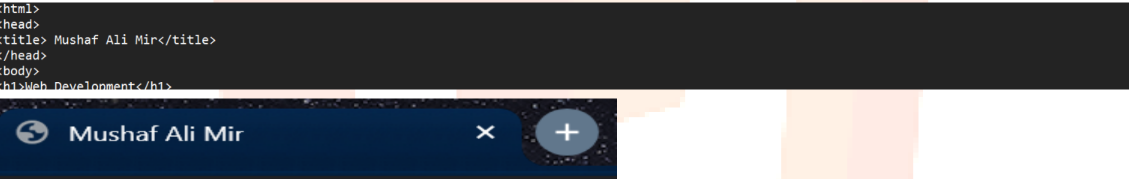
\includegraphics[width=0.8\linewidth]{8.1.png}
		\caption{Title Setup }
	\end{figure}
	STEP 1:-Create Html Tag and Head Tag.
	\begin{figure}[H]
		\centering
		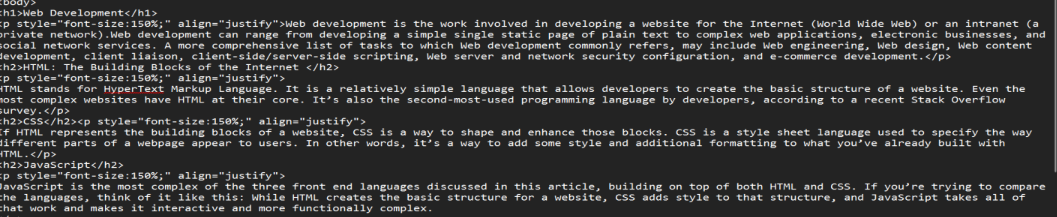
\includegraphics[width=0.8\linewidth]{8.2.png}
		\caption{HTML Head Tag}
	\end{figure}
	STEP 2:-Creating Body Tag And Paragraph tag.
	
	\begin{figure}[H]
		\centering
		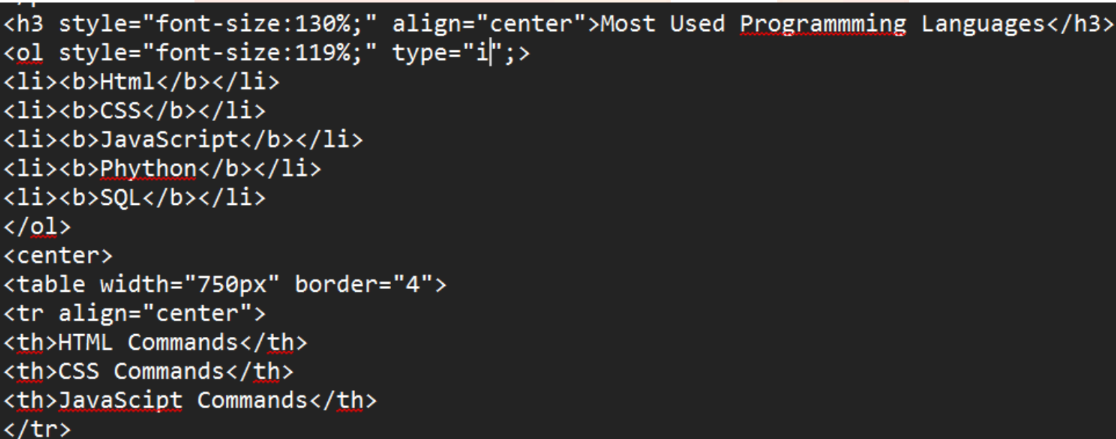
\includegraphics[width=0.8\linewidth]{8.3.png}
		\caption{Body And Paragraph Tag}
	\end{figure}
	STEP 3:-Creating List.
	\begin{figure}[H]
		\centering
		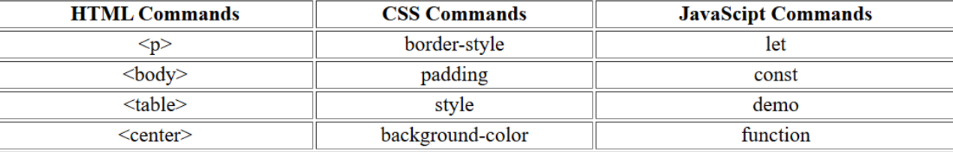
\includegraphics[width=0.8\linewidth]{8.4.png}
		\caption{Html Table}
	\end{figure}
	STEP 4:-Creating a table.
	\begin{figure}[H]
		\centering
		\includegraphics[width=0.8\linewidth]{8.5.png}
		\caption{My Webpage}
	\end{figure}
	STEP 5:-Final Result
	
\end{enumerate}

\subsection{Lab Task}

\begin{itemize}
	\item Write a basic HTML document with a title and body content..
	\item Add headings, paragraphs, and a list (ordered or unordered)..
	\item Include a hyperlink using the <a> tag.
	\item Embed an image using the <img> tag with appropriate attributes.
\end{itemize}

\subsection{Observation}
\begin{itemize}
	\item HTML commands allow the clear structuring of web content using tags.
	
	
	\item Proper nesting and closing of tags are crucial for rendering pages correctly.
	\item Links and multimedia elements enhance user interaction and experience.
	\item Simple forms enable data collection and basic user engagement.
\end{itemize}
\subsection{Conclusion}
HTML is an essential tool for creating and organizing web content. By mastering its commands and tags, developers can build static webpages that form the basis for advanced web applications. Understanding HTML commands enables efficient communication between developers and web browsers.

\subsection{Question}

\begin{enumerate}
	\item What is the significance of the <head> and <body> tags in an HTML document?
	
	\item How can hyperlinks be created and styled using the <a> tag?
	\item Describe the attributes required for embedding images with the <img> tag.
	\item Why is proper nesting of tags important in HTML?
	
\end{enumerate}

\newpage


%%%%%%%%%%%%%%%%%%%%%%%%%%%%%%%%%%%%%%%%%%%%%%%%5%%%%%%%%%%%%%%%%%%%%%%%%%%%%%%%%%%%%%%%%%%%%%%%%%%%%%%%%%%%%%%%%%%%%%%%%%%%%%%%%%%%%%%%%%%%%%%%%%%%%%%%%%%%%%%%%%%%%%%%%%%%%%%%%%%%%%%%%%%%%%%%%%%%%%%%%%%%%%%%%%%%%%%%%%%%%%%%%%%%%%%%%%%%%%%%%%%%5

\begin{center}
	{\Huge \bfseries \underline{ LAB ASSESSMENT 9: Javascript Forms } \par}
\end{center}
\noindent\begin{tabular}{@{}ll}
	\textbf{Lab title} :&Creating Forms With JavaScript \\
	\textbf{Course name} :&  Introduction to Information and Communication Technology\\
	\textbf{Author name} : & Mushaf Ali Mir\\
	\textbf{Submission date} :& 29 Nov 2024 \\
\end{tabular}

\section*{Introduction}
\addcontentsline{toc}{section}{9.   \hspace{1mm}Lab Task 9}
\setcounter{section}{9}
\setcounter{figure}{0}  % Set the section counter to 2
\setcounter{subsection}{0}

Creating interactive forms is a key aspect of web development. HTML provides the structure for form elements such as text fields, radio buttons, checkboxes, and submit buttons, while JavaScript enhances interactivity by validating user inputs and enabling dynamic functionality. This experiment focuses on designing forms using HTML and applying JavaScript to validate and process user input, ensuring better user experience and data accuracy.

\subsection{Objective}
The objective of this experiment is to learn how to create forms using HTML, integrate JavaScript for form validation and interactivity, and understand the importance of these tools in web development.

\subsection{Apparatus/Materials}
\begin{enumerate}
	\item Text editor (e.g., Visual Studio Code, Sublime Text)
	\item Web browser (e.g., Google Chrome, Mozilla Firefox)
	\item Computer with basic hardware and software support
	
\end{enumerate}
\subsection{Theory}
HTML forms are created using the \texttt{\textless form\textgreater} element, which serves as the container for all input elements such as \texttt{\textless input\textgreater}, \texttt{\textless textarea\textgreater}, \texttt{\textless select\textgreater}, and \texttt{\textless button\textgreater}. These elements enable users to input and submit data. JavaScript complements this setup by adding client-side validation to ensure that user inputs meet specified criteria before submission. For instance, JavaScript can verify email formats, ensure required fields are not left empty, and confirm password matching. Additionally, JavaScript provides dynamic interactivity, such as displaying error messages, enabling or disabling buttons, and giving real-time feedback. By combining HTML and JavaScript, developers can create efficient, user-friendly forms that enhance data accuracy and usability.

\subsection{Procedure}
\begin{enumerate}
	\item \textbf{Creating JavaScript Forms}
	
	\begin{figure}[H]
		\centering
		\includegraphics[width=0.8\linewidth]{9.1.png}
		\caption{Form Tag }
	\end{figure}
	STEP 1:-In this Section i have used html tag ’Form’ to create a form in my html page with this tag two input fields are
	generated for user to give input and the tag includes.
	Label
	Label tag to label our input fields in the html page.
	Input
	Input tag to create a input field for user to input data.
	\begin{figure}[H]
		\centering
		\includegraphics[width=0.8\linewidth]{9.2.png}
		\caption{JavaScript Functions}
	\end{figure}
	STEP 2:-In this section i have used the script tag to use Javascript and have made use of a function and the if and else
	structures to check weather the two input by the user are equal or not.
	Var
	In the code we have used var to declare a varible type which has global scope.
	Get element
	In by this function we get the value of the input by its ID.
	If–else
	By this function we do decision making thus by the output of true or false we give different outputs.
	
	\begin{figure}[H]
		\centering
		\includegraphics[width=0.8\linewidth]{9.3.png}
		\caption{My Web Page}
	\end{figure}
	STEP 3:-FINAL RESULT.
	
\end{enumerate}

\subsection{Lab Task}

\begin{itemize}
	\item Design a basic form using HTML: Include fields such as name, email, and password with the \texttt{\textless input\textgreater} element.
	\item Add dropdown menus and checkboxes: Use \texttt{\textless select\textgreater} and \texttt{\textless input type="checkbox"\textgreater} elements.
	\item Implement form validation using JavaScript: Validate email formats, check required fields, and provide error messages.
	\item Enable real-time feedback: Use JavaScript to show success or error messages dynamically.
\end{itemize}

\subsection{Observation}
\begin{itemize}
	\item HTML provides a clear and structured framework for creating forms using elements such as \texttt{\textless input\textgreater}, \texttt{\textless textarea\textgreater}, and \texttt{\textless button\textgreater}.
	
	
	\item JavaScript enhances forms by adding interactivity, enabling real-time validation, and improving user experience.
	\item Proper integration of HTML and JavaScript ensures seamless functionality.
\end{itemize}
\subsection{Conclusion}
This experiment highlights the importance of combining HTML and JavaScript to create interactive forms. HTML establishes the structural foundation, while JavaScript adds interactivity and validation, enabling effective and user-friendly web forms. Mastering these technologies is essential for modern web development.

\subsection{Question}

\begin{enumerate}
	\item What is the purpose of the \texttt{\textless form\textgreater} element in HTML?
	
	\item How does JavaScript validate user inputs before form submission?
	\item What attributes can be used with \texttt{\textless input\textgreater} to enhance form usability?.
	\item How can JavaScript provide real-time feedback during form interaction?
	
\end{enumerate}

\newpage


%%%%%%%%%%%%%%%%%%%%%%%%%%%%%%%%%%%%%%%%%%%%%%%%5%%%%%%%%%%%%%%%%%%%%%%%%%%%%%%%%%%%%%%%%%%%%%%%%%%%%%%%%%%%%%%%%%%%%%%%%%%%%%%%%%%%%%%%%%%%%%%%%%%%%%%%%%%%%%%%%%%%%%%%%%%%%%%%%%%%%%%%%%%%%%%%%%%%%%%%%%%%%%%%%%%%%%%%%%%%%%%%%%%%%%%%%%%%%%%%%%%%5

\begin{center}
	{\Huge \bfseries \underline{ LAB ASSESSMENT 10: Link Html Pages } \par}
\end{center}
\noindent\begin{tabular}{@{}ll}
	\textbf{Lab title} :&Linking Multiple Html Pages \\
	\textbf{Course name} :&  Introduction to Information and Communication Technology\\
	\textbf{Author name} : & Mushaf Ali Mir\\
	\textbf{Submission date} :& 30 Nov 2024 \\
\end{tabular}

\section*{Introduction}
\addcontentsline{toc}{section}{10.   \hspace{1mm}Lab Task 10}
\setcounter{section}{10}
\setcounter{figure}{0}  % Set the section counter to 2
\setcounter{subsection}{0}

Linking multiple pages in HTML is a fundamental concept in web development, enabling users to navigate seamlessly between different sections of a website. The \texttt{\textless a\textgreater} (anchor) tag is used to create hyperlinks that connect one page to another or to specific sections within a page. This experiment focuses on understanding the use of the \texttt{\textless a\textgreater} tag, working with the \texttt{href} attribute, and organizing multiple pages into a cohesive website structure.

\subsection{Objective}
The objective of this experiment is to learn how to link multiple HTML pages using the \texttt{\textless a\textgreater} tag, create navigation menus, and establish a logical flow between web pages.

\subsection{Apparatus/Materials}
\begin{enumerate}
	\item Text editor (e.g., Visual Studio Code, Sublime Text).
	\item Web browser (e.g., Google Chrome, Mozilla Firefox).
	\item Computer with basic hardware and software support
	
\end{enumerate}
\subsection{Theory}
Linking pages in HTML is achieved using the \texttt{\textless a\textgreater} tag, which defines a hyperlink. The \texttt{href} attribute specifies the location of the target page or resource. For example, \texttt{\textless a href="about.html"\textgreater About Us\textless /a\textgreater} links to a page named \texttt{about.html}. Links can be:

Relative links: Use file paths relative to the current document (e.g., \texttt{\textless a href="folder/page.html"\textgreater} for a file in a subfolder).
Absolute links: Use full URLs to link to external resources (e.g., \texttt{\textless a href="https://example.com"\textgreater}).
Additionally, navigation menus can be created using a list structure (\texttt{\textless ul\textgreater} and \texttt{\textless li\textgreater}) combined with multiple \texttt{\textless a\textgreater} tags. By linking multiple pages, developers can provide an intuitive user experience.

\subsection{Procedure}
\begin{enumerate}
	\item \textbf{Linking Html Pages}
	
	\begin{figure}[H]
		\centering
		\includegraphics[width=0.8\linewidth]{10.1.png}
		\caption{Page 1 }
	\end{figure}
	\begin{figure}[H]
		\centering
		\includegraphics[width=0.8\linewidth]{10.2.png}
		\caption{Page 2}
	\end{figure}
	
	\begin{figure}[H]
		\centering
		\includegraphics[width=0.8\linewidth]{10.3.png}
		\caption{Page 3}
	\end{figure}
	
	\begin{figure}[H]
		\centering
		\includegraphics[width=0.8\linewidth]{10.4.png}
		\caption{Page 4}
	\end{figure}
	
	The \texttt{\textless a\textgreater} tag is used to link different HTML pages. The syntax of the tag is:  
	\texttt{\textless a href="URL"\textgreater Text\textless /a\textgreater}  
	
	We use this tag to link multiple pages and create buttons to navigate between pages. The pages are designed with a background color using the tag:  
	\texttt{style="background-color: \#92A8D1;"}  
	
	The \texttt{\textless button\textgreater} tag in HTML is used to create clickable buttons that can perform actions.  
	
	The final result is shown below.
	
	
	
\end{enumerate}

\subsection{Lab Task}

\begin{itemize}
	\item Create three HTML pages (e.g., Home, About Us, and Contact Us).
	\item Link the pages together using the \texttt{\textless a\textgreater} tag:
	Add a navigation menu on each page with links to the other pages.
	Use relative paths for linking.
	\item Test the navigation to ensure all links are functional and correctly directed.
	\item Add anchor links within a single page to navigate between sections using IDs.
\end{itemize}

\subsection{Observation}
\begin{itemize}
	\item The \texttt{\textless a\textgreater} tag effectively links pages and provides smooth navigation.
	
	
	\item Navigation menus make websites user-friendly and organized.
	\item Proper use of relative paths simplifies linking within a project folder structure.
\end{itemize}
\subsection{Conclusion}
Linking multiple HTML pages is a core skill in building websites. The \texttt{\textless a\textgreater} tag enables seamless navigation, ensuring an organized and accessible website structure. By understanding relative and absolute linking methods, developers can efficiently create multi-page websites.

\subsection{Question}

\begin{enumerate}
	\item What is the purpose of the \texttt{\textless a\textgreater} tag in HTML?
	
	\item Explain the difference between relative and absolute links.
	
	\item Why is it important to structure your project files logically for linking?
	
	\item Describe how anchor links work within a single page.
	
\end{enumerate}

\newpage

%%%%%%%%%%%%%%%%%%%%%%%%%%%%%%%%%%%%%%%%%%%%%%%%5%%%%%%%%%%%%%%%%%%%%%%%%%%%%%%%%%%%%%%%%%%%%%%%%%%%%%%%%%%%%%%%%%%%%%%%%%%%%%%%%%%%%%%%%%%%%%%%%%%%%%%%%%%%%%%%%%%%%%%%%%%%%%%%%%%%%%%%%%%%%%%%%%%%%%%%%%%%%%%%%%%%%%%%%%%%%%%%%%%%%%%%%%%%%%%%%%%%5

\begin{center}
	{\Huge \bfseries \underline{ LAB ASSESSMENT 11: HTMl Login Page } \par}
\end{center}
\noindent\begin{tabular}{@{}ll}
	\textbf{Lab title} :& Creating Html Login Page \\
	\textbf{Course name} :&  Introduction to Information and Communication Technology\\
	\textbf{Author name} : & Mushaf Ali Mir\\
	\textbf{Submission date} :& 30 Nov 2024 \\
\end{tabular}

\section*{Introduction}
\addcontentsline{toc}{section}{11.   \hspace{1mm}Lab Task 11}
\setcounter{section}{11}
\setcounter{figure}{0}  % Set the section counter to 2
\setcounter{subsection}{0}

In web development, creating a login page is a crucial task for enabling user authentication. This experiment involves creating an HTML login page that includes username and password input fields. JavaScript is used to validate these credentials on the client side before submitting the form. This validation ensures the entered credentials match the predefined ones and provides real-time feedback to the user if they are incorrect.

\subsection{Objective}
The objective of this experiment is to design and implement a simple HTML login page and use JavaScript to validate the user credentials (username and password). The JavaScript code will check if the entered credentials match predefined values before submitting the form.

\subsection{Apparatus/Materials}
\begin{enumerate}
	\item Text editor (e.g., Visual Studio Code, Sublime Text)
	\item Web browser (e.g., Google Chrome, Mozilla Firefox)
	\item Computer with basic hardware and software support
	
\end{enumerate}
\subsection{Theory}
An HTML login page typically includes \texttt{\textless input\textgreater} fields for the username and password, organized within a \texttt{\textless form\textgreater} element. JavaScript is used to validate the input values. When the user submits the form, JavaScript ensures that the credentials match a predefined username and password. This helps to prevent incorrect data submission and enhances user experience by providing immediate feedback on failed attempts. The validation is performed in the browser, ensuring faster response times and less load on the server..

\subsection{Procedure}
\begin{enumerate}
	\item \textbf{Creating Slides Presentation}
	
	\begin{figure}[H]
		\centering
		\includegraphics[width=1\linewidth]{11.1.png}
		\caption{Form Tag}
	\end{figure}
	STEP 1:-\textless form\textgreater Tag
	The \textless form\textgreater tag is an HTML tag used to create a form (a square input field) for the user to enter data and information into.
	
	type: Specifies the type of input the form will accept.
	id: Assigns an ID to the input field, which can be referred to later for additional functionality and operations.
	script: The \textless script\textgreater tag is used to write JavaScript code and functionality within an HTML file.
	\begin{figure}[H]
		\centering
		\includegraphics[width=1\linewidth]{11.2.png}
		\caption{Windows Tag}
	\end{figure}
	STEP 2:-\texttt{\textless window.location.href = ("link")\textgreater}
	The \texttt{window.location} property is used to link pages together in a manner that allows each page to be directly accessed if specific conditions are met.
	
	\begin{figure}[H]
		\centering
		\includegraphics[width=0.6\linewidth]{11.3.png}
		\caption{Login Page}
	\end{figure}
	\begin{figure}[H]
		\centering
		\includegraphics[width=0.8\linewidth]{11.4.png}
		\caption{Successful Access}
	\end{figure}
.
	\begin{figure}[H]
		\centering
		\includegraphics[width=0.8\linewidth]{11.5.png}
		\caption{Failed Access}
	\end{figure}
  Final Linked Login Pages.
\end{enumerate}

\subsection{Lab Task}

\begin{itemize}
	\item \texttt{\textless} Create an HTML login page \textgreater with two input fields for the username and password.
	\item \texttt{\textless} Use JavaScript to validate \textgreater if the entered credentials match predefined values (e.g., username: "admin", password: "password123").
	\item \texttt{\textless} Display an alert or message \textgreater if the login fails, instructing the user to try again.
	
	\item \texttt{\textless} Ensure the page does not reload \textgreater unless the credentials are correct.
	
\end{itemize}

\subsection{Observation}
\begin{itemize}
	\item The HTML page correctly displays the input fields and the login button.
	
	
	\item JavaScript validation runs when the user clicks the submit button, checking if the entered credentials match the expected values.
	.
	\item If the credentials are incorrect, the page shows a validation message or alert, as intended..
	\item The form only submits successfully when valid credentials are entered.
\end{itemize}
\subsection{Conclusion}
Creating a login page using HTML and JavaScript for client-side validation enhances the user experience by providing immediate feedback on incorrect credentials. This experiment successfully demonstrated how JavaScript can be used to validate user input on the client side before form submission.
\subsection{Question}

\begin{enumerate}
	\item What is the purpose of client-side validation in a login form?
	
	\item How can you modify the JavaScript code to allow multiple sets of usernames and passwords?
	\item Explain why it's important to not rely solely on client-side validation for security.
	\item How could you improve this login page to store and retrieve credentials securely?
	
\end{enumerate}

\newpage


	    
\end{document}
